\documentclass[10pt]{article} % For LaTeX2e
\usepackage[preprint]{tmlr}
% If accepted, instead use the following line for the camera-ready submission:
%\usepackage[accepted]{tmlr}
% To de-anonymize and remove mentions to TMLR (for example for posting to preprint servers), instead use the following:
%\usepackage[preprint]{tmlr}

% Optional math commands from https://github.com/goodfeli/dlbook_notation.
%%%%% NEW MATH DEFINITIONS %%%%%

\usepackage{amsmath,amsfonts,bm}

% Mark sections of captions for referring to divisions of figures
\newcommand{\figleft}{{\em (Left)}}
\newcommand{\figcenter}{{\em (Center)}}
\newcommand{\figright}{{\em (Right)}}
\newcommand{\figtop}{{\em (Top)}}
\newcommand{\figbottom}{{\em (Bottom)}}
\newcommand{\captiona}{{\em (a)}}
\newcommand{\captionb}{{\em (b)}}
\newcommand{\captionc}{{\em (c)}}
\newcommand{\captiond}{{\em (d)}}

% Highlight a newly defined term
\newcommand{\newterm}[1]{{\bf #1}}


% Figure reference, lower-case.
\def\figref#1{figure~\ref{#1}}
% Figure reference, capital. For start of sentence
\def\Figref#1{Figure~\ref{#1}}
\def\twofigref#1#2{figures \ref{#1} and \ref{#2}}
\def\quadfigref#1#2#3#4{figures \ref{#1}, \ref{#2}, \ref{#3} and \ref{#4}}
% Section reference, lower-case.
\def\secref#1{section~\ref{#1}}
% Section reference, capital.
\def\Secref#1{Section~\ref{#1}}
% Reference to two sections.
\def\twosecrefs#1#2{sections \ref{#1} and \ref{#2}}
% Reference to three sections.
\def\secrefs#1#2#3{sections \ref{#1}, \ref{#2} and \ref{#3}}
% Reference to an equation, lower-case.
\def\eqref#1{equation~\ref{#1}}
% Reference to an equation, upper case
\def\Eqref#1{Equation~\ref{#1}}
% A raw reference to an equation---avoid using if possible
\def\plaineqref#1{\ref{#1}}
% Reference to a chapter, lower-case.
\def\chapref#1{chapter~\ref{#1}}
% Reference to an equation, upper case.
\def\Chapref#1{Chapter~\ref{#1}}
% Reference to a range of chapters
\def\rangechapref#1#2{chapters\ref{#1}--\ref{#2}}
% Reference to an algorithm, lower-case.
\def\algref#1{algorithm~\ref{#1}}
% Reference to an algorithm, upper case.
\def\Algref#1{Algorithm~\ref{#1}}
\def\twoalgref#1#2{algorithms \ref{#1} and \ref{#2}}
\def\Twoalgref#1#2{Algorithms \ref{#1} and \ref{#2}}
% Reference to a part, lower case
\def\partref#1{part~\ref{#1}}
% Reference to a part, upper case
\def\Partref#1{Part~\ref{#1}}
\def\twopartref#1#2{parts \ref{#1} and \ref{#2}}

\def\ceil#1{\lceil #1 \rceil}
\def\floor#1{\lfloor #1 \rfloor}
\def\1{\bm{1}}
\newcommand{\train}{\mathcal{D}}
\newcommand{\valid}{\mathcal{D_{\mathrm{valid}}}}
\newcommand{\test}{\mathcal{D_{\mathrm{test}}}}

\def\eps{{\epsilon}}


% Random variables
\def\reta{{\textnormal{$\eta$}}}
\def\ra{{\textnormal{a}}}
\def\rb{{\textnormal{b}}}
\def\rc{{\textnormal{c}}}
\def\rd{{\textnormal{d}}}
\def\re{{\textnormal{e}}}
\def\rf{{\textnormal{f}}}
\def\rg{{\textnormal{g}}}
\def\rh{{\textnormal{h}}}
\def\ri{{\textnormal{i}}}
\def\rj{{\textnormal{j}}}
\def\rk{{\textnormal{k}}}
\def\rl{{\textnormal{l}}}
% rm is already a command, just don't name any random variables m
\def\rn{{\textnormal{n}}}
\def\ro{{\textnormal{o}}}
\def\rp{{\textnormal{p}}}
\def\rq{{\textnormal{q}}}
\def\rr{{\textnormal{r}}}
\def\rs{{\textnormal{s}}}
\def\rt{{\textnormal{t}}}
\def\ru{{\textnormal{u}}}
\def\rv{{\textnormal{v}}}
\def\rw{{\textnormal{w}}}
\def\rx{{\textnormal{x}}}
\def\ry{{\textnormal{y}}}
\def\rz{{\textnormal{z}}}

% Random vectors
\def\rvepsilon{{\mathbf{\epsilon}}}
\def\rvtheta{{\mathbf{\theta}}}
\def\rva{{\mathbf{a}}}
\def\rvb{{\mathbf{b}}}
\def\rvc{{\mathbf{c}}}
\def\rvd{{\mathbf{d}}}
\def\rve{{\mathbf{e}}}
\def\rvf{{\mathbf{f}}}
\def\rvg{{\mathbf{g}}}
\def\rvh{{\mathbf{h}}}
\def\rvu{{\mathbf{i}}}
\def\rvj{{\mathbf{j}}}
\def\rvk{{\mathbf{k}}}
\def\rvl{{\mathbf{l}}}
\def\rvm{{\mathbf{m}}}
\def\rvn{{\mathbf{n}}}
\def\rvo{{\mathbf{o}}}
\def\rvp{{\mathbf{p}}}
\def\rvq{{\mathbf{q}}}
\def\rvr{{\mathbf{r}}}
\def\rvs{{\mathbf{s}}}
\def\rvt{{\mathbf{t}}}
\def\rvu{{\mathbf{u}}}
\def\rvv{{\mathbf{v}}}
\def\rvw{{\mathbf{w}}}
\def\rvx{{\mathbf{x}}}
\def\rvy{{\mathbf{y}}}
\def\rvz{{\mathbf{z}}}

% Elements of random vectors
\def\erva{{\textnormal{a}}}
\def\ervb{{\textnormal{b}}}
\def\ervc{{\textnormal{c}}}
\def\ervd{{\textnormal{d}}}
\def\erve{{\textnormal{e}}}
\def\ervf{{\textnormal{f}}}
\def\ervg{{\textnormal{g}}}
\def\ervh{{\textnormal{h}}}
\def\ervi{{\textnormal{i}}}
\def\ervj{{\textnormal{j}}}
\def\ervk{{\textnormal{k}}}
\def\ervl{{\textnormal{l}}}
\def\ervm{{\textnormal{m}}}
\def\ervn{{\textnormal{n}}}
\def\ervo{{\textnormal{o}}}
\def\ervp{{\textnormal{p}}}
\def\ervq{{\textnormal{q}}}
\def\ervr{{\textnormal{r}}}
\def\ervs{{\textnormal{s}}}
\def\ervt{{\textnormal{t}}}
\def\ervu{{\textnormal{u}}}
\def\ervv{{\textnormal{v}}}
\def\ervw{{\textnormal{w}}}
\def\ervx{{\textnormal{x}}}
\def\ervy{{\textnormal{y}}}
\def\ervz{{\textnormal{z}}}

% Random matrices
\def\rmA{{\mathbf{A}}}
\def\rmB{{\mathbf{B}}}
\def\rmC{{\mathbf{C}}}
\def\rmD{{\mathbf{D}}}
\def\rmE{{\mathbf{E}}}
\def\rmF{{\mathbf{F}}}
\def\rmG{{\mathbf{G}}}
\def\rmH{{\mathbf{H}}}
\def\rmI{{\mathbf{I}}}
\def\rmJ{{\mathbf{J}}}
\def\rmK{{\mathbf{K}}}
\def\rmL{{\mathbf{L}}}
\def\rmM{{\mathbf{M}}}
\def\rmN{{\mathbf{N}}}
\def\rmO{{\mathbf{O}}}
\def\rmP{{\mathbf{P}}}
\def\rmQ{{\mathbf{Q}}}
\def\rmR{{\mathbf{R}}}
\def\rmS{{\mathbf{S}}}
\def\rmT{{\mathbf{T}}}
\def\rmU{{\mathbf{U}}}
\def\rmV{{\mathbf{V}}}
\def\rmW{{\mathbf{W}}}
\def\rmX{{\mathbf{X}}}
\def\rmY{{\mathbf{Y}}}
\def\rmZ{{\mathbf{Z}}}

% Elements of random matrices
\def\ermA{{\textnormal{A}}}
\def\ermB{{\textnormal{B}}}
\def\ermC{{\textnormal{C}}}
\def\ermD{{\textnormal{D}}}
\def\ermE{{\textnormal{E}}}
\def\ermF{{\textnormal{F}}}
\def\ermG{{\textnormal{G}}}
\def\ermH{{\textnormal{H}}}
\def\ermI{{\textnormal{I}}}
\def\ermJ{{\textnormal{J}}}
\def\ermK{{\textnormal{K}}}
\def\ermL{{\textnormal{L}}}
\def\ermM{{\textnormal{M}}}
\def\ermN{{\textnormal{N}}}
\def\ermO{{\textnormal{O}}}
\def\ermP{{\textnormal{P}}}
\def\ermQ{{\textnormal{Q}}}
\def\ermR{{\textnormal{R}}}
\def\ermS{{\textnormal{S}}}
\def\ermT{{\textnormal{T}}}
\def\ermU{{\textnormal{U}}}
\def\ermV{{\textnormal{V}}}
\def\ermW{{\textnormal{W}}}
\def\ermX{{\textnormal{X}}}
\def\ermY{{\textnormal{Y}}}
\def\ermZ{{\textnormal{Z}}}

% Vectors
\def\vzero{{\bm{0}}}
\def\vone{{\bm{1}}}
\def\vmu{{\bm{\mu}}}
\def\vtheta{{\bm{\theta}}}
\def\va{{\bm{a}}}
\def\vb{{\bm{b}}}
\def\vc{{\bm{c}}}
\def\vd{{\bm{d}}}
\def\ve{{\bm{e}}}
\def\vf{{\bm{f}}}
\def\vg{{\bm{g}}}
\def\vh{{\bm{h}}}
\def\vi{{\bm{i}}}
\def\vj{{\bm{j}}}
\def\vk{{\bm{k}}}
\def\vl{{\bm{l}}}
\def\vm{{\bm{m}}}
\def\vn{{\bm{n}}}
\def\vo{{\bm{o}}}
\def\vp{{\bm{p}}}
\def\vq{{\bm{q}}}
\def\vr{{\bm{r}}}
\def\vs{{\bm{s}}}
\def\vt{{\bm{t}}}
\def\vu{{\bm{u}}}
\def\vv{{\bm{v}}}
\def\vw{{\bm{w}}}
\def\vx{{\bm{x}}}
\def\vy{{\bm{y}}}
\def\vz{{\bm{z}}}

% Elements of vectors
\def\evalpha{{\alpha}}
\def\evbeta{{\beta}}
\def\evepsilon{{\epsilon}}
\def\evlambda{{\lambda}}
\def\evomega{{\omega}}
\def\evmu{{\mu}}
\def\evpsi{{\psi}}
\def\evsigma{{\sigma}}
\def\evtheta{{\theta}}
\def\eva{{a}}
\def\evb{{b}}
\def\evc{{c}}
\def\evd{{d}}
\def\eve{{e}}
\def\evf{{f}}
\def\evg{{g}}
\def\evh{{h}}
\def\evi{{i}}
\def\evj{{j}}
\def\evk{{k}}
\def\evl{{l}}
\def\evm{{m}}
\def\evn{{n}}
\def\evo{{o}}
\def\evp{{p}}
\def\evq{{q}}
\def\evr{{r}}
\def\evs{{s}}
\def\evt{{t}}
\def\evu{{u}}
\def\evv{{v}}
\def\evw{{w}}
\def\evx{{x}}
\def\evy{{y}}
\def\evz{{z}}

% Matrix
\def\mA{{\bm{A}}}
\def\mB{{\bm{B}}}
\def\mC{{\bm{C}}}
\def\mD{{\bm{D}}}
\def\mE{{\bm{E}}}
\def\mF{{\bm{F}}}
\def\mG{{\bm{G}}}
\def\mH{{\bm{H}}}
\def\mI{{\bm{I}}}
\def\mJ{{\bm{J}}}
\def\mK{{\bm{K}}}
\def\mL{{\bm{L}}}
\def\mM{{\bm{M}}}
\def\mN{{\bm{N}}}
\def\mO{{\bm{O}}}
\def\mP{{\bm{P}}}
\def\mQ{{\bm{Q}}}
\def\mR{{\bm{R}}}
\def\mS{{\bm{S}}}
\def\mT{{\bm{T}}}
\def\mU{{\bm{U}}}
\def\mV{{\bm{V}}}
\def\mW{{\bm{W}}}
\def\mX{{\bm{X}}}
\def\mY{{\bm{Y}}}
\def\mZ{{\bm{Z}}}
\def\mBeta{{\bm{\beta}}}
\def\mPhi{{\bm{\Phi}}}
\def\mLambda{{\bm{\Lambda}}}
\def\mSigma{{\bm{\Sigma}}}

% Tensor
\DeclareMathAlphabet{\mathsfit}{\encodingdefault}{\sfdefault}{m}{sl}
\SetMathAlphabet{\mathsfit}{bold}{\encodingdefault}{\sfdefault}{bx}{n}
\newcommand{\tens}[1]{\bm{\mathsfit{#1}}}
\def\tA{{\tens{A}}}
\def\tB{{\tens{B}}}
\def\tC{{\tens{C}}}
\def\tD{{\tens{D}}}
\def\tE{{\tens{E}}}
\def\tF{{\tens{F}}}
\def\tG{{\tens{G}}}
\def\tH{{\tens{H}}}
\def\tI{{\tens{I}}}
\def\tJ{{\tens{J}}}
\def\tK{{\tens{K}}}
\def\tL{{\tens{L}}}
\def\tM{{\tens{M}}}
\def\tN{{\tens{N}}}
\def\tO{{\tens{O}}}
\def\tP{{\tens{P}}}
\def\tQ{{\tens{Q}}}
\def\tR{{\tens{R}}}
\def\tS{{\tens{S}}}
\def\tT{{\tens{T}}}
\def\tU{{\tens{U}}}
\def\tV{{\tens{V}}}
\def\tW{{\tens{W}}}
\def\tX{{\tens{X}}}
\def\tY{{\tens{Y}}}
\def\tZ{{\tens{Z}}}


% Graph
\def\gA{{\mathcal{A}}}
\def\gB{{\mathcal{B}}}
\def\gC{{\mathcal{C}}}
\def\gD{{\mathcal{D}}}
\def\gE{{\mathcal{E}}}
\def\gF{{\mathcal{F}}}
\def\gG{{\mathcal{G}}}
\def\gH{{\mathcal{H}}}
\def\gI{{\mathcal{I}}}
\def\gJ{{\mathcal{J}}}
\def\gK{{\mathcal{K}}}
\def\gL{{\mathcal{L}}}
\def\gM{{\mathcal{M}}}
\def\gN{{\mathcal{N}}}
\def\gO{{\mathcal{O}}}
\def\gP{{\mathcal{P}}}
\def\gQ{{\mathcal{Q}}}
\def\gR{{\mathcal{R}}}
\def\gS{{\mathcal{S}}}
\def\gT{{\mathcal{T}}}
\def\gU{{\mathcal{U}}}
\def\gV{{\mathcal{V}}}
\def\gW{{\mathcal{W}}}
\def\gX{{\mathcal{X}}}
\def\gY{{\mathcal{Y}}}
\def\gZ{{\mathcal{Z}}}

% Sets
\def\sA{{\mathbb{A}}}
\def\sB{{\mathbb{B}}}
\def\sC{{\mathbb{C}}}
\def\sD{{\mathbb{D}}}
% Don't use a set called E, because this would be the same as our symbol
% for expectation.
\def\sF{{\mathbb{F}}}
\def\sG{{\mathbb{G}}}
\def\sH{{\mathbb{H}}}
\def\sI{{\mathbb{I}}}
\def\sJ{{\mathbb{J}}}
\def\sK{{\mathbb{K}}}
\def\sL{{\mathbb{L}}}
\def\sM{{\mathbb{M}}}
\def\sN{{\mathbb{N}}}
\def\sO{{\mathbb{O}}}
\def\sP{{\mathbb{P}}}
\def\sQ{{\mathbb{Q}}}
\def\sR{{\mathbb{R}}}
\def\sS{{\mathbb{S}}}
\def\sT{{\mathbb{T}}}
\def\sU{{\mathbb{U}}}
\def\sV{{\mathbb{V}}}
\def\sW{{\mathbb{W}}}
\def\sX{{\mathbb{X}}}
\def\sY{{\mathbb{Y}}}
\def\sZ{{\mathbb{Z}}}

% Entries of a matrix
\def\emLambda{{\Lambda}}
\def\emA{{A}}
\def\emB{{B}}
\def\emC{{C}}
\def\emD{{D}}
\def\emE{{E}}
\def\emF{{F}}
\def\emG{{G}}
\def\emH{{H}}
\def\emI{{I}}
\def\emJ{{J}}
\def\emK{{K}}
\def\emL{{L}}
\def\emM{{M}}
\def\emN{{N}}
\def\emO{{O}}
\def\emP{{P}}
\def\emQ{{Q}}
\def\emR{{R}}
\def\emS{{S}}
\def\emT{{T}}
\def\emU{{U}}
\def\emV{{V}}
\def\emW{{W}}
\def\emX{{X}}
\def\emY{{Y}}
\def\emZ{{Z}}
\def\emSigma{{\Sigma}}

% entries of a tensor
% Same font as tensor, without \bm wrapper
\newcommand{\etens}[1]{\mathsfit{#1}}
\def\etLambda{{\etens{\Lambda}}}
\def\etA{{\etens{A}}}
\def\etB{{\etens{B}}}
\def\etC{{\etens{C}}}
\def\etD{{\etens{D}}}
\def\etE{{\etens{E}}}
\def\etF{{\etens{F}}}
\def\etG{{\etens{G}}}
\def\etH{{\etens{H}}}
\def\etI{{\etens{I}}}
\def\etJ{{\etens{J}}}
\def\etK{{\etens{K}}}
\def\etL{{\etens{L}}}
\def\etM{{\etens{M}}}
\def\etN{{\etens{N}}}
\def\etO{{\etens{O}}}
\def\etP{{\etens{P}}}
\def\etQ{{\etens{Q}}}
\def\etR{{\etens{R}}}
\def\etS{{\etens{S}}}
\def\etT{{\etens{T}}}
\def\etU{{\etens{U}}}
\def\etV{{\etens{V}}}
\def\etW{{\etens{W}}}
\def\etX{{\etens{X}}}
\def\etY{{\etens{Y}}}
\def\etZ{{\etens{Z}}}

% The true underlying data generating distribution
\newcommand{\pdata}{p_{\rm{data}}}
% The empirical distribution defined by the training set
\newcommand{\ptrain}{\hat{p}_{\rm{data}}}
\newcommand{\Ptrain}{\hat{P}_{\rm{data}}}
% The model distribution
\newcommand{\pmodel}{p_{\rm{model}}}
\newcommand{\Pmodel}{P_{\rm{model}}}
\newcommand{\ptildemodel}{\tilde{p}_{\rm{model}}}
% Stochastic autoencoder distributions
\newcommand{\pencode}{p_{\rm{encoder}}}
\newcommand{\pdecode}{p_{\rm{decoder}}}
\newcommand{\precons}{p_{\rm{reconstruct}}}

\newcommand{\laplace}{\mathrm{Laplace}} % Laplace distribution

\newcommand{\E}{\mathbb{E}}
\newcommand{\Ls}{\mathcal{L}}
\newcommand{\R}{\mathbb{R}}
\newcommand{\emp}{\tilde{p}}
\newcommand{\lr}{\alpha}
\newcommand{\reg}{\lambda}
\newcommand{\rect}{\mathrm{rectifier}}
\newcommand{\softmax}{\mathrm{softmax}}
\newcommand{\sigmoid}{\sigma}
\newcommand{\softplus}{\zeta}
\newcommand{\KL}{D_{\mathrm{KL}}}
\newcommand{\Var}{\mathrm{Var}}
\newcommand{\standarderror}{\mathrm{SE}}
\newcommand{\Cov}{\mathrm{Cov}}
% Wolfram Mathworld says $L^2$ is for function spaces and $\ell^2$ is for vectors
% But then they seem to use $L^2$ for vectors throughout the site, and so does
% wikipedia.
\newcommand{\normlzero}{L^0}
\newcommand{\normlone}{L^1}
\newcommand{\normltwo}{L^2}
\newcommand{\normlp}{L^p}
\newcommand{\normmax}{L^\infty}

\newcommand{\parents}{Pa} % See usage in notation.tex. Chosen to match Daphne's book.

\DeclareMathOperator*{\argmax}{arg\,max}
\DeclareMathOperator*{\argmin}{arg\,min}

\DeclareMathOperator{\sign}{sign}
\DeclareMathOperator{\Tr}{Tr}
\let\ab\allowbreak


\usepackage{url}
\usepackage{graphicx}
\usepackage{array}
\usepackage{booktabs}
\usepackage{lipsum}
\usepackage{xspace}
\usepackage{pdflscape} 
\usepackage{multirow} 
\usepackage{listings}

% Custom colors
\usepackage{color}
\definecolor{deepblue}{rgb}{0,0,0.5}
\definecolor{deepred}{rgb}{0.6,0,0}
\definecolor{deepgreen}{rgb}{0,0.5,0}

\definecolor{xlinkcolor}{rgb}{0.7752941176470588, 0.22078431372549023, 0.2262745098039215}
\definecolor{codegreen}{rgb}{0,0.6,0}
\definecolor{codegray}{rgb}{0.5,0.5,0.5}
\definecolor{codepurple}{rgb}{0.58,0,0.82}
\definecolor{backcolour}{rgb}{0.95,0.95,0.92}

\newcommand{\package}[1]{\textsl{#1}\xspace}
\newcommand{\eg}{{e.\,g.}\xspace}
\newcommand{\ie}{{i.\,e.}\xspace}
\newcommand{\SM}[1]{\textcolor{blue}{[SM: #1]}}
\newcommand{\hubble}{\emph{Hubble}\xspace}

\def\preprintno{XXXX} % Insert correct preprint number

\usepackage[
pdfnewwindow=true,      % links in new window
colorlinks=true,    % false: boxed links; true: colored links
linkcolor=xlinkcolor,     % color of internal links
citecolor=xlinkcolor,     % color of links to bibliography
filecolor=xlinkcolor,  % color of file links
urlcolor=xlinkcolor,      % color of external links
final=true,
]{hyperref}

% Define a new fancy page style
\fancypagestyle{firstpage}{
    \rhead{MIT-CTP/\preprintno}
    % Define other header and footer elements if necessary
}

\lstdefinestyle{mystyle}{
  backgroundcolor=\color{backcolour},
  commentstyle=\color{codegreen},
  keywordstyle=\color{magenta},
  numberstyle=\tiny\color{codegray},
  stringstyle=\color{codegreen},
  basicstyle=\ttfamily\footnotesize,
  breakatwhitespace=false,
  breaklines=true,
  captionpos=b,
  keepspaces=true,
  numbers=left,
  numbersep=5pt,
  showspaces=false,
  showstringspaces=false,
  showtabs=false,
  frame=single, % adds a frame around the code
  rulecolor=\color{black}, % if you want to change the frame color
  tabsize=2
}

\lstset{style=mystyle}

\title{\textsc{HubbleCLIP}: Associating Astronomical Observations and Natural Language with Multi-Modal Models}

% Authors must not appear in the submitted version. They should be hidden
% as long as the tmlr package is used without the [accepted] or [preprint] options.
% Non-anonymous submissions will be rejected without review.

\author{\name Siddharth Mishra-Sharma \email \href{mailto:smsharma@mit.edu}{smsharma@mit.edu} \\
      \addr The NSF AI Institute for Artificial Intelligence and Fundamental Interactions\\
      Center for Theoretical Physics, Massachusetts Institute of Technology, Cambridge, MA 02139, USA \\
      Department of Physics, Harvard University, Cambridge, MA 02138, USA
      \AND
      \name Yiding Song \email \href{mailto:ydsong@mit.edu}{ydsong@mit.edu} \\
      \addr The NSF AI Institute for Artificial Intelligence and Fundamental Interactions\\
      Department of Physics, Massachusetts Institute of Technology, Cambridge, MA 02139, USA \\
      \AND
      \name Jesse Thaler \email \href{mailto:jthaler@mit.edu}{jthaler@mit.edu} \\
      \addr The NSF AI Institute for Artificial Intelligence and Fundamental Interactions\\
      Center for Theoretical Physics, Massachusetts Institute of Technology, Cambridge, MA 02139, USA \\
}
% The \author macro works with any number of authors. Use \AND 
% to separate the names and addresses of multiple authors.

\newcommand{\fix}{\marginpar{FIX}}
\newcommand{\new}{\marginpar{NEW}}

\def\month{MM}  % Insert correct month for camera-ready version
\def\year{YYYY} % Insert correct year for camera-ready version
\def\openreview{\url{https://openreview.net/forum?id=XXXX}} % Insert correct link to OpenReview for camera-ready version

\newcommand{\datafolder}[1]{\def\thedatafolder{#1}}


\begin{document}


\maketitle

\thispagestyle{firstpage}

\begin{abstract}
We present a multi-modal model which associates astronomical observations imaged by the \hubble Space Telescope (HST) with natural language. The model is fine-tuned from a base CLIP model using successful proposal abstracts corresponding to HST observations, summarized via guided large language (LLM) model generation. We show that the model embodies a meaningful joint representation between observations and text through experiments targeting observation retrieval (i.e., retrieving the most relevant observations from a set using natural language queries) and description retrieval (i.e., querying the astrophysical object classes and science use cases most relevant to a given observation). The model demonstrates the potential for using generalist rather than task-specific models for astrophysics research, in particular by leveraging text as an interface.
\end{abstract}

\section{Introduction}
\label{sec:intro}

Machine learning (ML) is starting to have a significant impact on the sciences, with astrophysics being no exception. Machine learning methods have demonstrated promise when applied to every part of the astrophysics pipeline, from instrument design, to data acquisition, to its analysis. Until recently, most applications of ML within astrophysics have focused on replacing or augmenting traditional techniques with ML counterparts in order to improve performance on specific tasks.

The \emph{Foundation Model} paradigm, in contrast, seeks to develop generalist models which can be deployed on a wide range of tasks. The paradigm has been highly successful in domains like computer vision and natural language processing, as demonstrated by the widespread adoption of tools like CLIP, ChatGPT, Dall-E, and Stable Diffusion. These models are typically pre-trained on massive amounts of unlabeled data using self-supervised learning techniques, enabling them to learn powerful representations which can be optionally fine-tuned to address domain-specific tasks. At the heart of the paradigm lies the triumph of scale -- scaling up model size, dataset size, and compute. However, foundation models often benefit from fine tuning using a relatively small amounts of domain-specific data, increasing their usefulness when applied to those specific domains.

There is considerable interest in developing custom foundation models for the sciences, with astrophysics being ripe for such an effort due to several reasons. The first is the availability of large amounts of publicly-available data as a contingency of publicy-funded data-taking efforts. The second is the multi-modality inherent astrophysical observations, with different types of data (e.g., images, spectra, light curves, textual descriptions) often available for each observation. This multi-modality was recently exploited to train \textsc{AstroCLIP}~\citep{lanusse2023astroclip} -- a joint representation between multi-band images and optical spectra from the Dark Energy Spectroscopic Instrument (DESI). \textsc{AstroLLaMA}~\citep{nguyen2023astrollama} is another recent effort to fine-tune a publicly-available model (\textsc{Llama-2}) on astrophysics-specific textual data from the arXiv.

The CLIP~\citep{radford2021learning} family of models has shown strong performance on a variety of downstream tasks including zero-shot classification and image retrieval.

\textsc{GeoCLIP}~\citep{cepeda2023geoclip}.

The success of the foundation model paradigm partly relies on the ability to flexibly leverage text as a \emph{universal interface}. In this work, we take this outlook and train a joint representation between observations taken by the \hubble Space Telescope (HST) and natural language. We do so by using the associations between observation proposals and corresponding downstream observations. We show that fine-tuning a CLIP (Contrastive Language-Image Pre-training) model on this data enables learning meaningful joint representations.

The paper is organized as follows. In Sec.~\ref{sec:dataset}, we describe the dataset used in this work, including its curation and processing. In Sec.~\ref{sec:methodology}, we describe the methodology used to train and evaluate the model. In Sec.~\ref{sec:results}, we present the results of our experiments on image and text retrieval tasks. We discuss future prospects and conclude in Sec.~\ref{sec:conclusion}.

\section{Dataset Construction}
\label{sec:dataset}

We curate a dataset of images of \hubble observations and corresponding text descriptions. We rely on summarized versions of proposal abstracts from the Proposal Abstracts Catalog\footnote{\url{https://archive.stsci.edu/hst/proposal_abstracts.html}} -- a catalog of all accepted \hubble proposals -- to derive captions for the observations. The HST has been operational for 33 years, having been launched on April 24, 1990. We use available proposals and observations up to Cycle 30, which commenced data-taking in 2022. 

Examples of images and corresponding captions are shown in Tab.~\ref{tab:dataset}. It can be seen that these images have specific characteristics as well as artifacts particular to the nature of data-taking which distinguish them from the distribution of natural images typically used for large-scale pre-training of foundation models. This further motivates the need for fine-tuning on domain-specific data.

\subsection{Data Selection and Pre-processing}

Observations corresponding to individual proposal IDs are queried through the Mikulski Archive for Space Telescopes (MAST) via the \texttt{astroquery} interface. Products of type \texttt{PREVIEW} are filtered in, corresponding to preview postcard images. Note that these are not science-grade observations, but rather low-resolution images used for quick-look purposes; given the nature of associations we aim to learn, we deem this adequate for our current purposes. A maximum of 20 images are downloaded per proposal ID, selected at random, in order to avoid biasing the model towards proposals with a larger number of observations. Images are centered and resized to a resolution per side of 512 pixels before saving. Color previews (i.e., observations taken with multiple wavelength filters assigned to individual RGB channels) are manually excluded via a filename filter in order to maintain consistency across the dataset; models trained on datasets with color images included were observed to show worse performance on generalization metrics. If no appropriate images corresponding to an abstract are found, the abstract is excluded from the dataset.

In total 31,859 images corresponding to 4,438 abstracts are included in the fine-tuning dataset. 3,194 images are held out for validation, with no abstract being common between training and validation sets in order to ensure an independent set of text-image pairs for testing.

% Mention that the signal is noisy!

\subsection{Summarization via Guided Generation}
\label{sec:summarization}

Raw abstracts summarize the corresponding successful HST observing proposals, which intend to make the case for allocating \hubble telescope time towards a particular set of observations. These abstracts are written in a diversity of styles, formats, and lengths, being highly variable in the nature of content as well. Although the abstracts can be used as-is as image captions, we explore the use of summarization via guided LLM generation to standardize the captions used for fine-tuning the CLIP model. The goal is to summarize the objects and phenomena, as well as potential downstream science use cases corresponding to the HST observations in order to increase the signal between text and images.

The method from \cite{willard2023efficient} is used to produce an LLM-generated summary of the abstract conforming to a particular schema, specified in JSON format. The schema is designed to represent a list of the objects (e.g., `Type Ia supernova') and phenomena (e.g., `gravitational lensing'), as well as potential downstream science uses cases (e.g., `set constraints on supernova explosion models') that could correspond to the eventual imaged observation given the abstract text.

The procedure guides the generation of LLM outputs while ensuring that the schema is respected at every point in the generation by masking out tokens that would violate the intended format. By framing the problem in terms of transitions between a set of finite-state machines, \cite{willard2023efficient} showed that guided generation can be performed with negligible overhead compared to unconstrained generation. This ensures that the output of the LLM strictly conforms to the format of the following example:
\begin{lstlisting}[language=Python]
{
  'objects_and_phenomena': ['star forming galaxy', 'lensed galaxy', ...], 
  'science_use_cases': ['measure lensing magnification', 'probe spectral energy distributions', ...]
}
\end{lstlisting}
which is then used to construct the summarized caption by combining the two key elements. Examples of raw abstracts and corresponding LLM-generated summaries are shown in Tab.~\ref{tab:datasetsumm}. Further details on the summarization procedure, including the prompts used and a more detailed description of guided generation, are provided in App.~\ref{app:summarization}.

The open-weights, instruction-tuned model \textsc{Mixtral-8x7B}\footnote{\url{https://huggingface.co/mistralai/Mixtral-8x7B-Instruct-v0.1}} is used to generate the summaries, with guided generation performed using the \texttt{outlines}\footnote{\url{https://github.com/outlines-dev/outlines}} package.

The goal if summarization-via-guided-generation is to increase the signal between text and images by standardizing the captions used for fine-tuning the CLIP model. 

% Note that the signal is very imperfect!

\datafolder{./plots/data/}
 
\begin{table}[h!]
      \centering
      \begin{tabular}{m{0.21\textwidth} p{1.9cm} p{1.9cm} m{8cm}}
          \toprule
          \centering \bfseries Image & \centering \bfseries Obs. cycle & \centering \bfseries Prop. ID & \centering \bfseries LLM-extracted summary \tabularnewline
          \midrule
          \centering 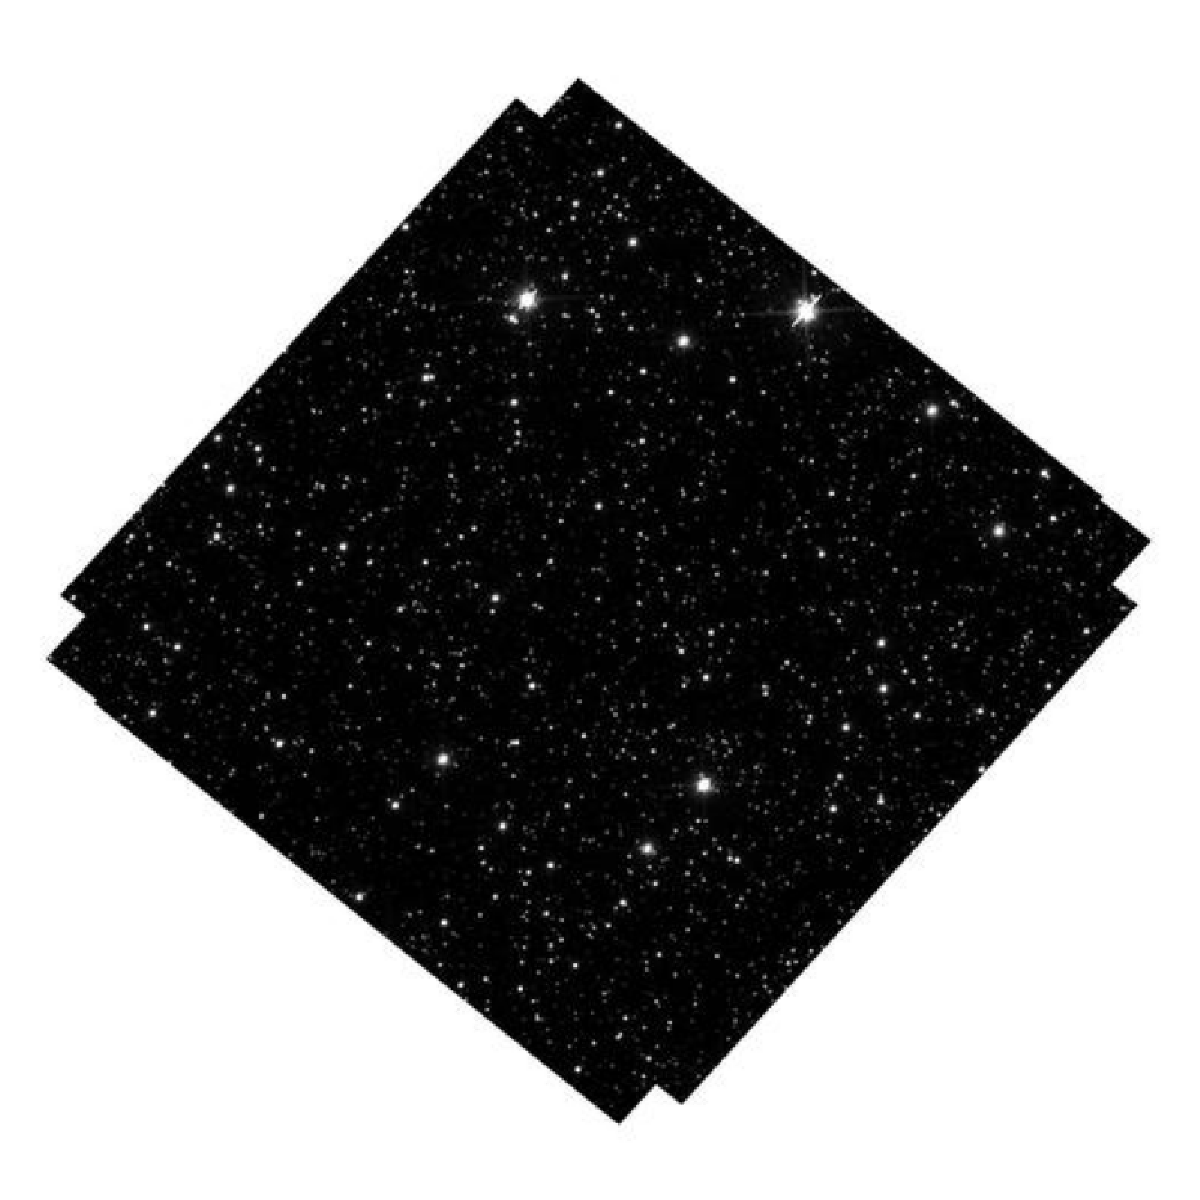
\includegraphics[width=0.2\textwidth]{\thedatafolder/img_0.pdf} & \centering \input{\thedatafolder/cycle_0.txt} & \centering \input{\thedatafolder/id_0.txt} &  {\scriptsize \input{\thedatafolder/sum_0.txt}} \tabularnewline
          \midrule
          \centering 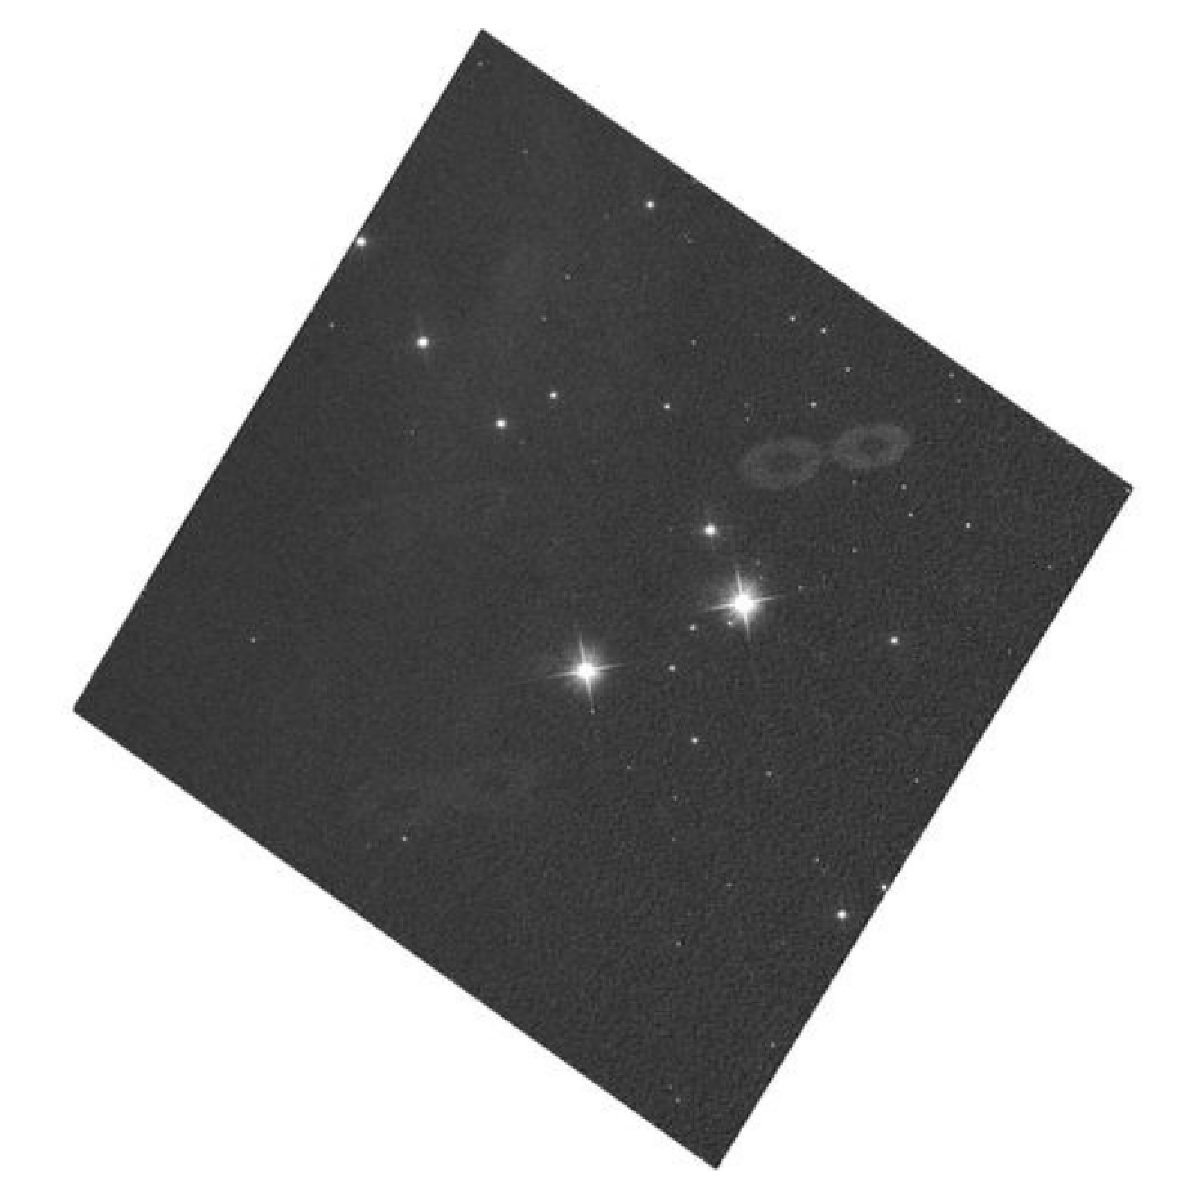
\includegraphics[width=0.2\textwidth]{\thedatafolder/img_1.pdf} & \centering \input{\thedatafolder/cycle_1.txt} & \centering \input{\thedatafolder/id_1.txt} &  {\scriptsize \input{\thedatafolder/sum_1.txt}} \tabularnewline
          \midrule
          \centering 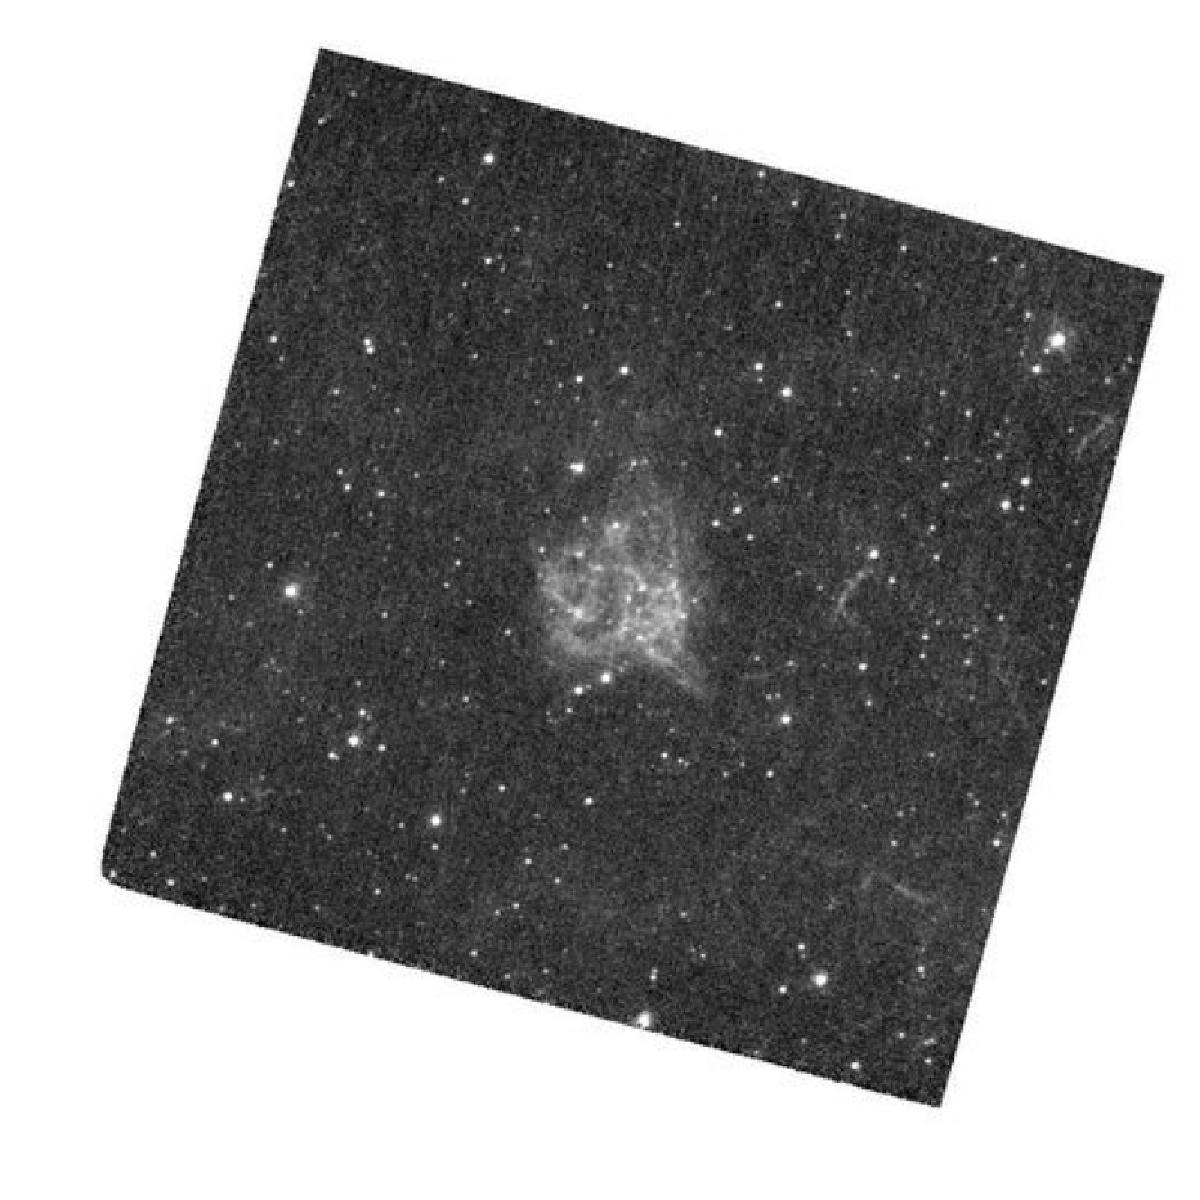
\includegraphics[width=0.2\textwidth]{\thedatafolder/img_2.pdf} & \centering \input{\thedatafolder/cycle_2.txt} & \centering \input{\thedatafolder/id_2.txt} &  {\scriptsize \input{\thedatafolder/sum_2.txt}} \tabularnewline
          \midrule
          \centering 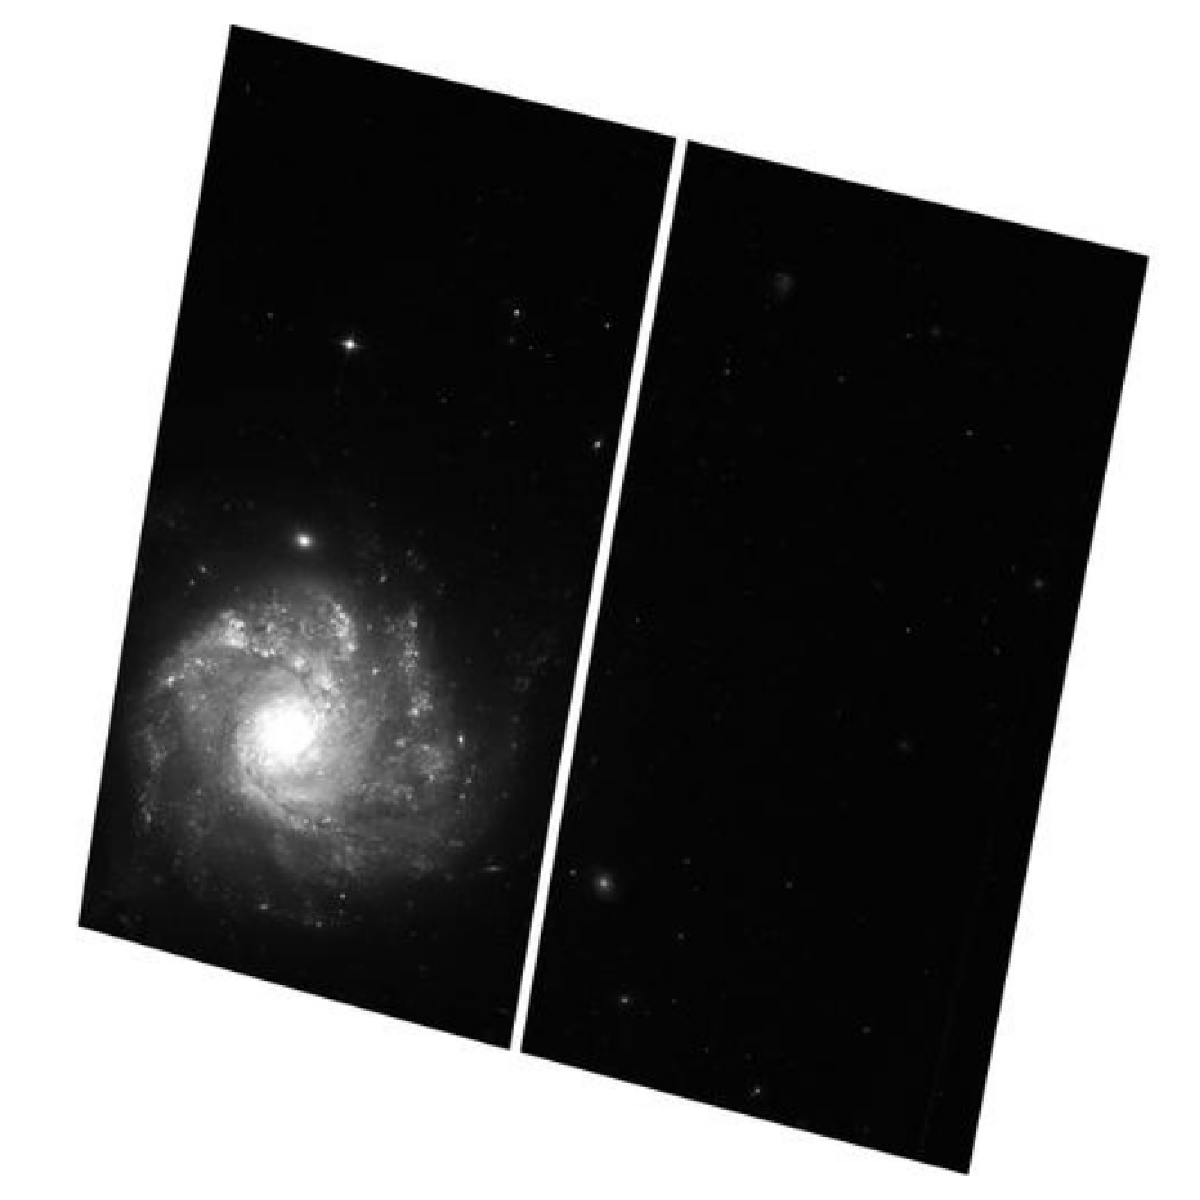
\includegraphics[width=0.2\textwidth]{\thedatafolder/img_3.pdf} & \centering \input{\thedatafolder/cycle_3.txt} & \centering \input{\thedatafolder/id_3.txt} &  {\scriptsize \input{\thedatafolder/sum_3.txt}} \tabularnewline
          \bottomrule
      \end{tabular}
      \caption{Examples of images and corresponding captions, constructed using the LLM-extracted summaries. The CLIP model is fine-tuned on these text-image associations.}
      \label{tab:dataset}
  \end{table}

\begin{landscape}
      \begin{table}[h!]
          \centering
          \begin{tabular}{m{1.8cm} m{8cm} m{5cm} m{6cm}}
              \toprule
              \bfseries Prop. ID & \centering\arraybackslash \bfseries Proposal abstract & \multicolumn{2}{c}{\bfseries LLM-extracted summary} \tabularnewline
              \cmidrule(r){3-4}
              & & \centering\arraybackslash \bfseries Objects and phenomena & \centering\arraybackslash \bfseries Science use cases \tabularnewline
              \midrule
              \input{\thedatafolder/id1_0.txt} & {\scriptsize \input{\thedatafolder/abs1_0.txt}} & {\scriptsize \input{\thedatafolder/obj1_0.txt}} & {\scriptsize \input{\thedatafolder/sci1_0.txt}} \tabularnewline
              \midrule
              \input{\thedatafolder/id1_1.txt} & {\scriptsize \input{\thedatafolder/abs1_1.txt}} & {\scriptsize \input{\thedatafolder/obj1_1.txt}} & {\scriptsize \input{\thedatafolder/sci1_1.txt}} \tabularnewline
              \midrule
              \input{\thedatafolder/id1_2.txt} & {\scriptsize \input{\thedatafolder/abs1_2.txt}} & {\scriptsize \input{\thedatafolder/obj1_2.txt}} & {\scriptsize \input{\thedatafolder/sci1_2.txt}} \tabularnewline
              \midrule
              \input{\thedatafolder/id1_3.txt} & {\scriptsize \input{\thedatafolder/abs1_3.txt}} & {\scriptsize \input{\thedatafolder/obj1_3.txt}} & {\scriptsize \input{\thedatafolder/sci1_3.txt}} \tabularnewline
              \bottomrule
          \end{tabular}
          \caption{Examples of the initial parts of raw proposal abstracts (second column) and LLM (\textsc{Mixtral-8x7B})-extracted summaries (rightmost two columns), separately extracting objects and phenomena as well as potential downstream science use cases. The LLM-extracted summaries are used for associating text with observations.}
          \label{tab:datasetsumm}
      \end{table}
  \end{landscape}

\section{Methodology}
\label{sec:methodology}

Our goal is to learn a semantically  meaningful joint representation of HST image observations and natural language, with the intention of using it for a variety of downstream tasks. We leverage the strong generalization capabilities demonstrated by CLIP (Contrastive Language-Image Pretraining) and adapt these to work with domain-specific \hubble data via fine-tuning; we describe these below.

\subsection{Language-Image Pre-training}
\label{sec:pretraining}

CLIP \citep[Contrastive Language-Image Pretraining;][]{radford2021learning} is a multi-modal model pre-trained on a large corpus of image-text pairs via weak supervision using a contrastive loss. Given a minibatch $\mathcal{B}$ of $|\mathcal{B}|$ image-text pairs $\{(I_i, T_i)\}$, the goal is to align the learned representations of corresponding (positive) pairs $(I_i, T_i)$ while repelling the representations of unaligned (negative) pairs $(I_i, T_{j\neq i})$. Image and text encoders $f(\cdot)$ and $g(\cdot)$ are used to map images and text to a common embedding space. The standard softmax-based bidirectional variation of the InfoNCE~\citep{oord2018representation} contrastive loss function, as used by CLIP, is particularly effective for multimodal learning. This bidirectionality is crucial as it ensures the model learns to map both images to text and text to images with equal importance. This symmetry in learning is essential for tasks that require a mutual understanding and interchangeability between visual and textual representations, such as image captioning, text-to-image synthesis, and cross-modal retrieval. The bidirectional loss is given by \citep{radford2021learning}
\begin{equation}
\mathcal L(\mathcal B) = -\frac{1}{2|\mathcal{B}|} \sum_{i=1}^{|\mathcal{B}|}\left(\overbrace{\log \frac{e^{{x}_i \cdot {y}_i / \tau}}{\sum_{j=1}^{|\mathcal{B}|} e^{{x}_i \cdot {y}_j / \tau}}}^{\text {image } \rightarrow \text { text softmax }}+\overbrace{\log \frac{e^{{x}_i \cdot {y}_i / \tau}}{\sum_{j=1}^{|\mathcal{B}|} e^{{x}_j \cdot {y}_i / \tau}}}^{\text {text } \rightarrow \text { image softmax }}\right)
\end{equation}
where ${x}_i=\frac{f\left(I_i\right)}{\left\|f\left(I_i\right)\right\|_2}$ and ${y}_i=\frac{g\left(T_i\right)}{\left\|g\left(T_i\right)\right\|_2}$ are the normalized representations of the $i$-th image and text, respectively, and $\tau$ is a (typically learnable) temperature hyperparameter. This bidirectional approach not only enhances the model's ability to create robust and versatile embeddings but also aligns with the intuitive understanding of how humans interact with and interpret multimodal information, further bridging the gap between artificial and natural intelligence in multimodal contexts.

As the base model, we use the CLIP-ViT-B/16 \citep{radford2021learning} variant trained by OpenAI. This model uses a (12-layer, 12-head, 768-embedding dimension) vision transformer as the image encoder and a (12-layer, 8-head, 512-embedding dimension) sequence transformer as the text backbone. The text encoder has a maximum length of 77-tokens and the image encoder a native resolution of $224\times224$. Linear projection layers map the outputs of the image and text encoders to a common embedding space of dimension 512. In total, the model has 149,620,737 trainable parameters. The model was trained on 400 million image-text pairs from the internet. 

\subsection{Fine-tuning Procedure and Evaluation}
\label{sec:finetuning}

The base CLIP model is fine-tuned using the dataset described in Sec.~\ref{sec:dataset}, using either the LLM-summarized data or the raw proposal abstracts. When using raw proposal abstracts, random chunks of the text delimited by periods are selected on the fly to fit within the maximum token length of the text encoder. Images are randomly cropped to the native resolution of the image encoder and randomly rotated at each training step. Given the relatively modest size of the fine-tuning set, a batch size $|\mathcal B| = 32$ is used throughout. We note that the positive and negative image-text association is noisy and imperfect, since multiple images can be associated with the same abstract.

We explore three different methods of training the model on our domain dataset: \emph{(1)} Fine-tuning the entire network, starting from the pre-trained base model; \emph{(2)} Freezing the base image and text encoders, and training a small projection head on top of these; and \emph{(3)} Training the entire model from scratch.

The model is trained over 50,000 steps with 5000 linear warmup steps and cosine decay using the AdamW optimizer \citep{DBLP:conf/iclr/LoshchilovH19,DBLP:journals/corr/KingmaB14} with peak learning rate of either $10^{-5}$ or $10^{-6}$ and weight decay $10^{-3}$. Training takes approximately 6 hours on 4 Nvidia A100 GPUs.

\section{Results and Discussion}
\label{sec:results}

% Effect of using summarization
% Effect of using a base model vs fine-tuning from scratch

\subsection{Fine-tuned Retrieval Accuracy}
\label{sec:retrieval_acc}

\subsection{`Zero-shot' Hypothesis and Object Retrieval}
\label{sec:zero_shot}

\subsection{Text-to-Image Retrieval}
\label{sec:tti}

\section{Outlook and Conclusions}
\label{sec:conclusion}

% \begin{figure*}[!h]
% \includegraphics[width=0.95\textwidth]{example-image-a}
% \caption{Overview of dataset}
% \label{fig:dataset}
% \end{figure*}


  

\begin{figure*}[!h]
      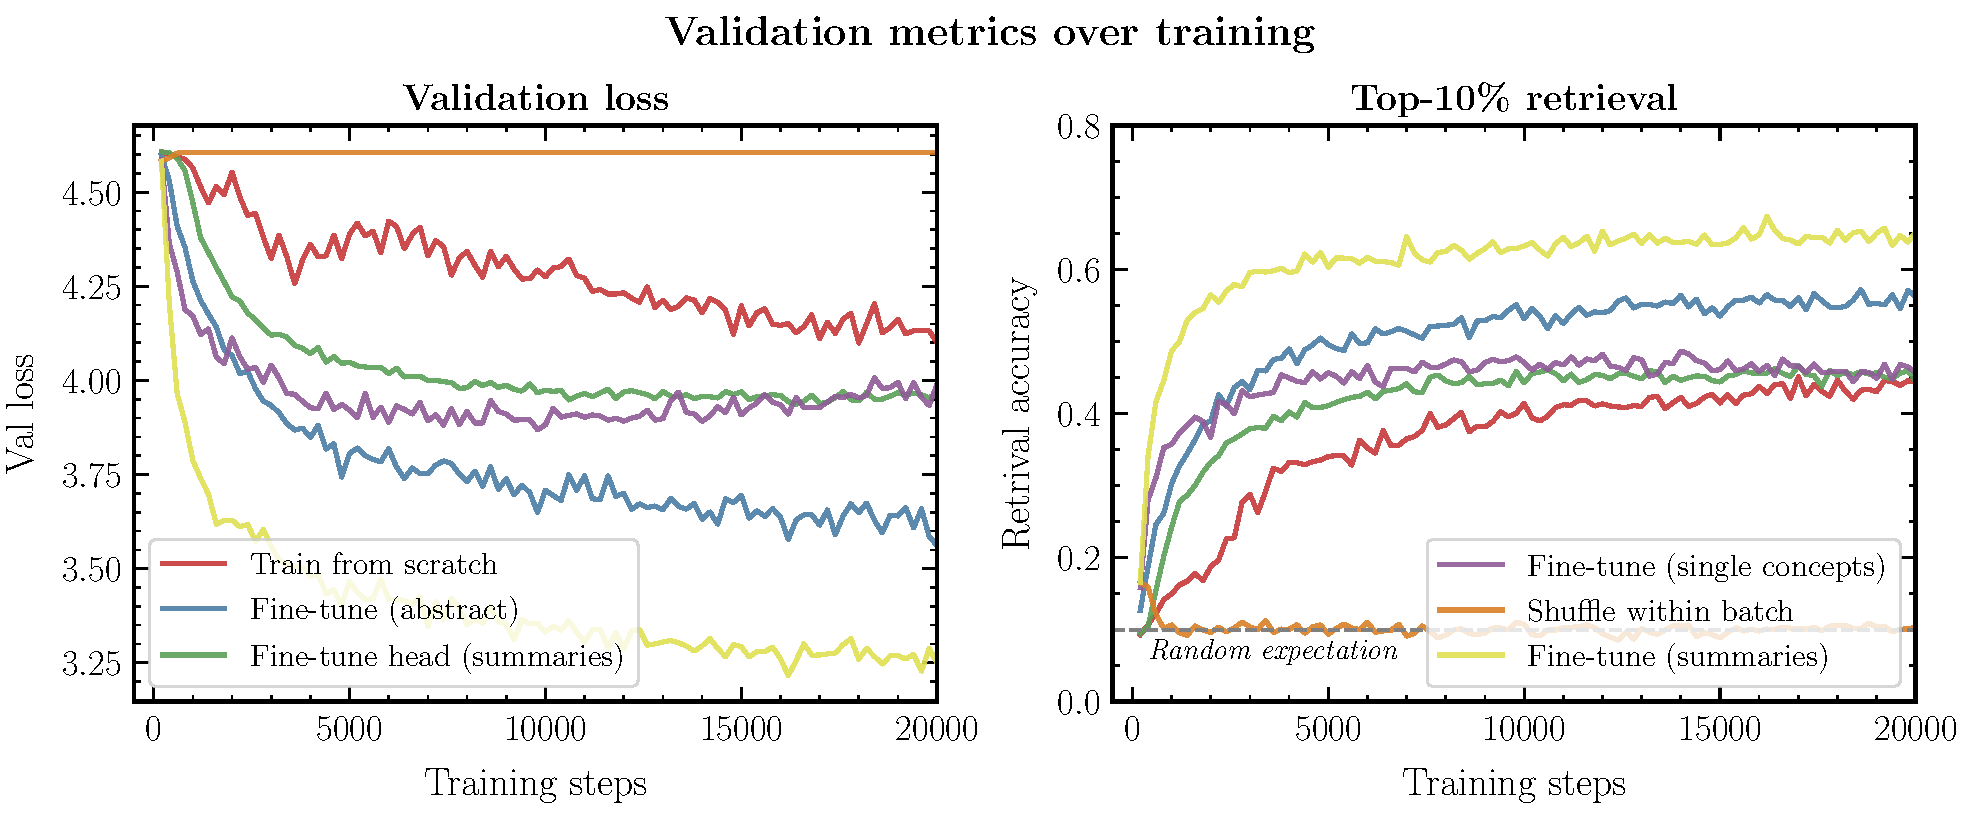
\includegraphics[width=0.95\textwidth]{plots/val_metrics.pdf}
      \caption{Retrieval accuracy}
      \label{fig:retrieval_acc}
      \end{figure*}
      

\begin{figure*}[!h]
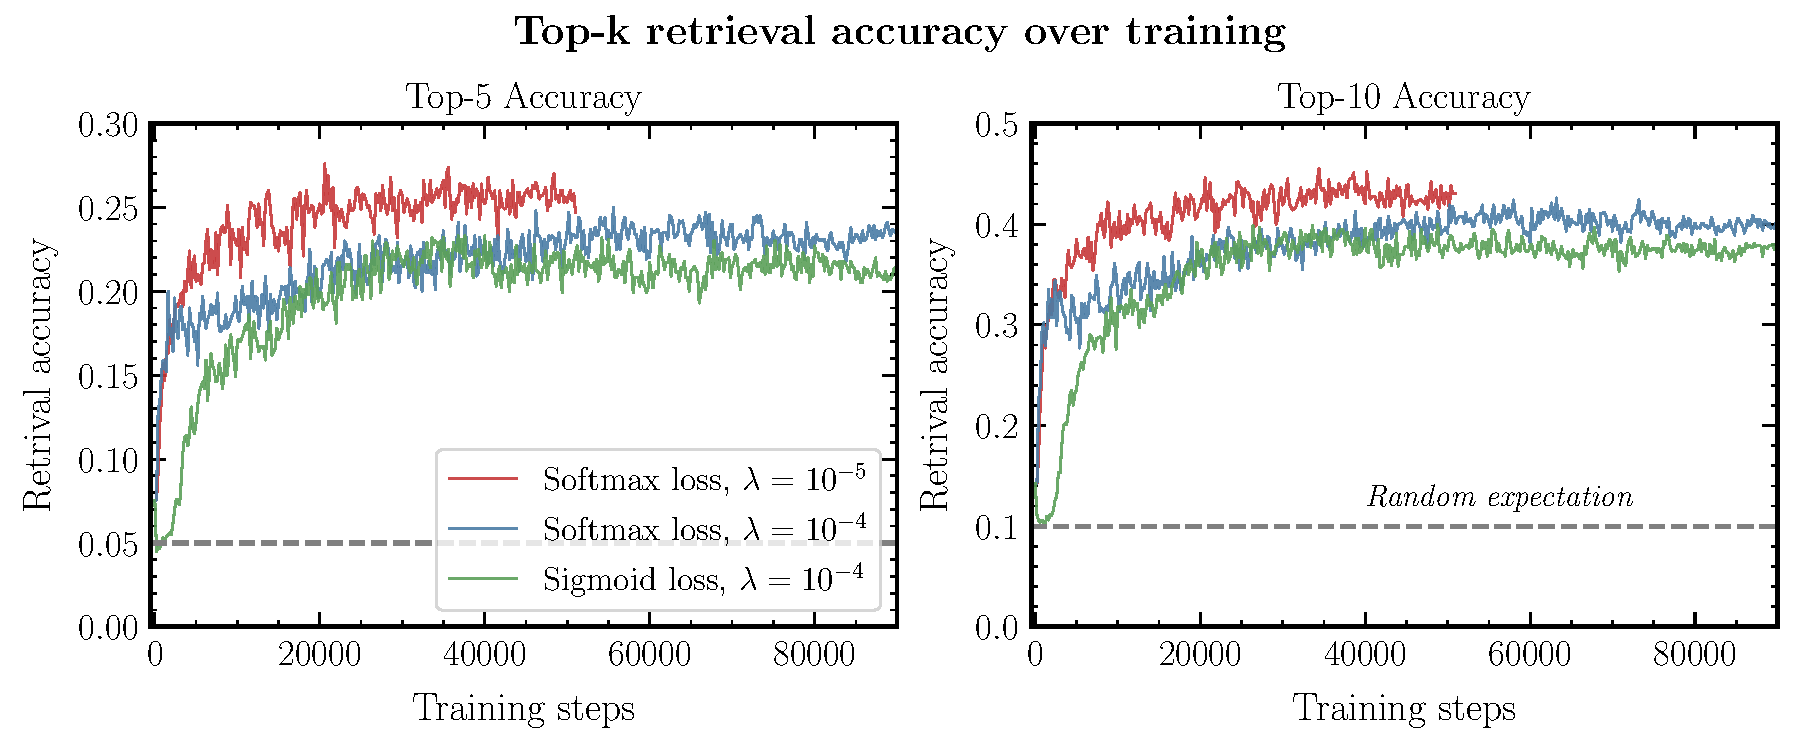
\includegraphics[width=0.95\textwidth]{plots/retrieval_acc.pdf}
\caption{Retrieval accuracy}
\label{fig:retrieval_acc}
\end{figure*}

\begin{figure*}[!h]
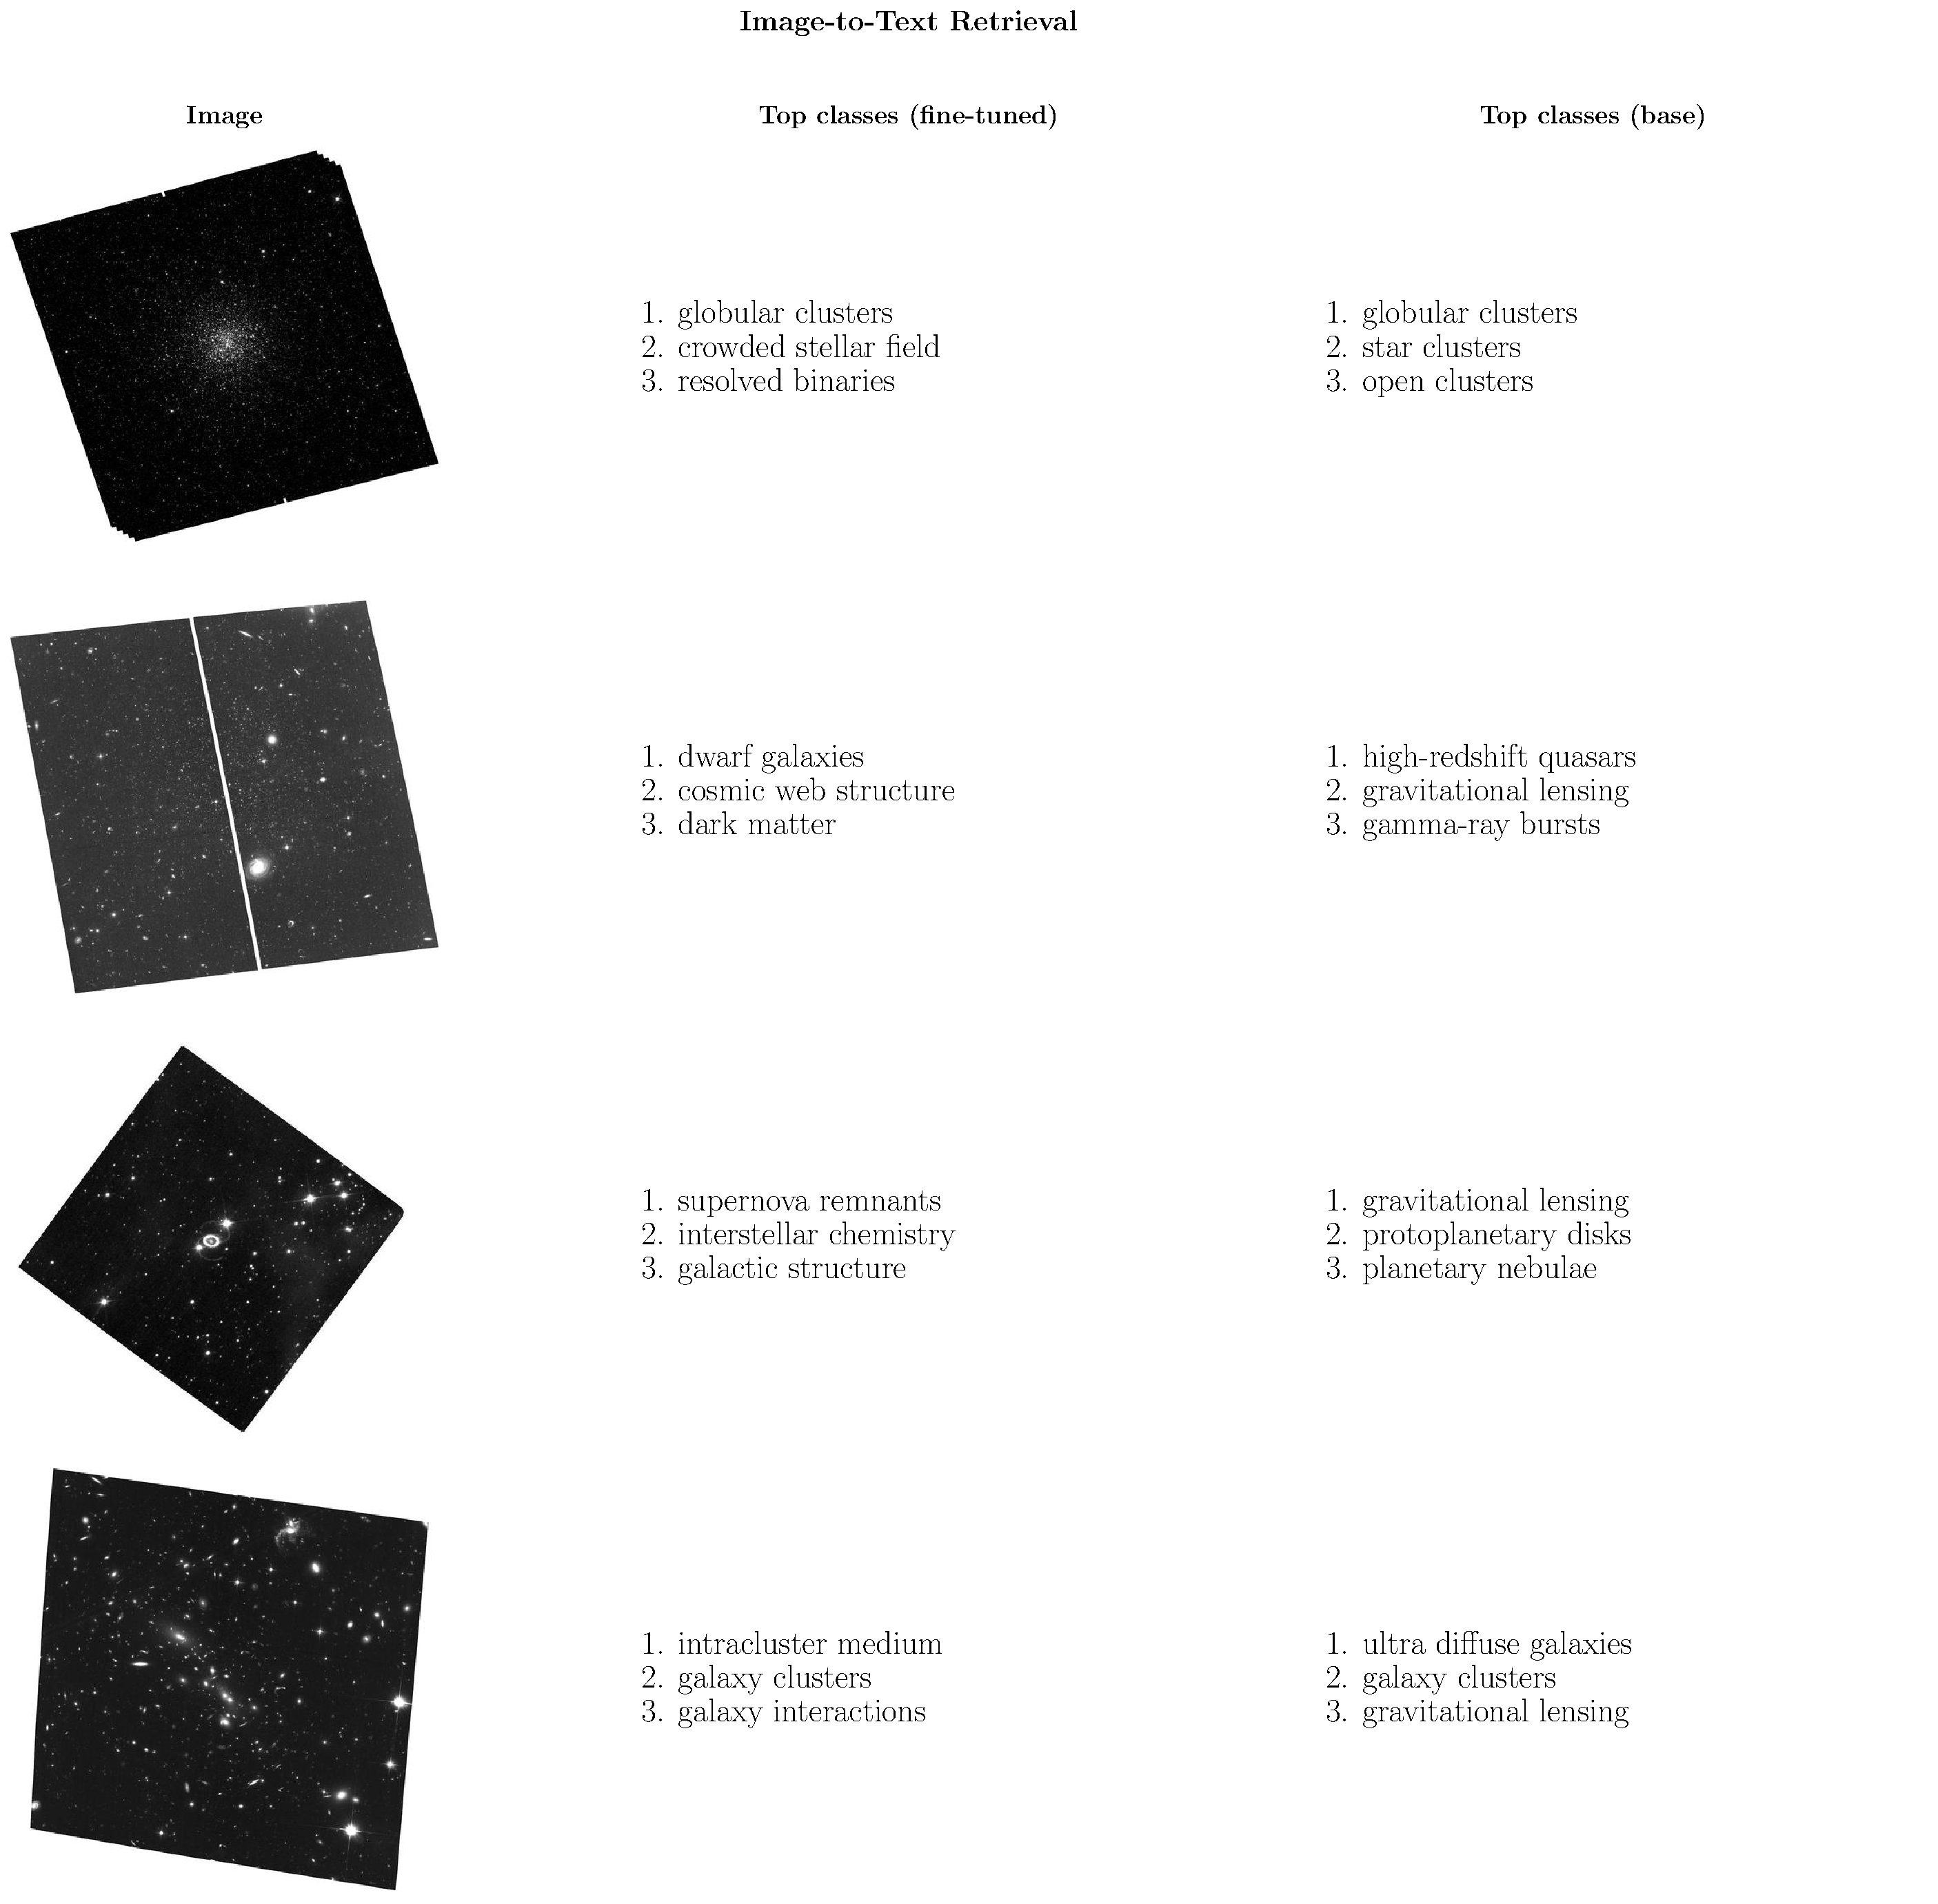
\includegraphics[width=0.95\textwidth]{plots/itt.pdf}
\caption{Retrieval accuracy}
\label{fig:itt}
\end{figure*}

\begin{figure*}[!h]
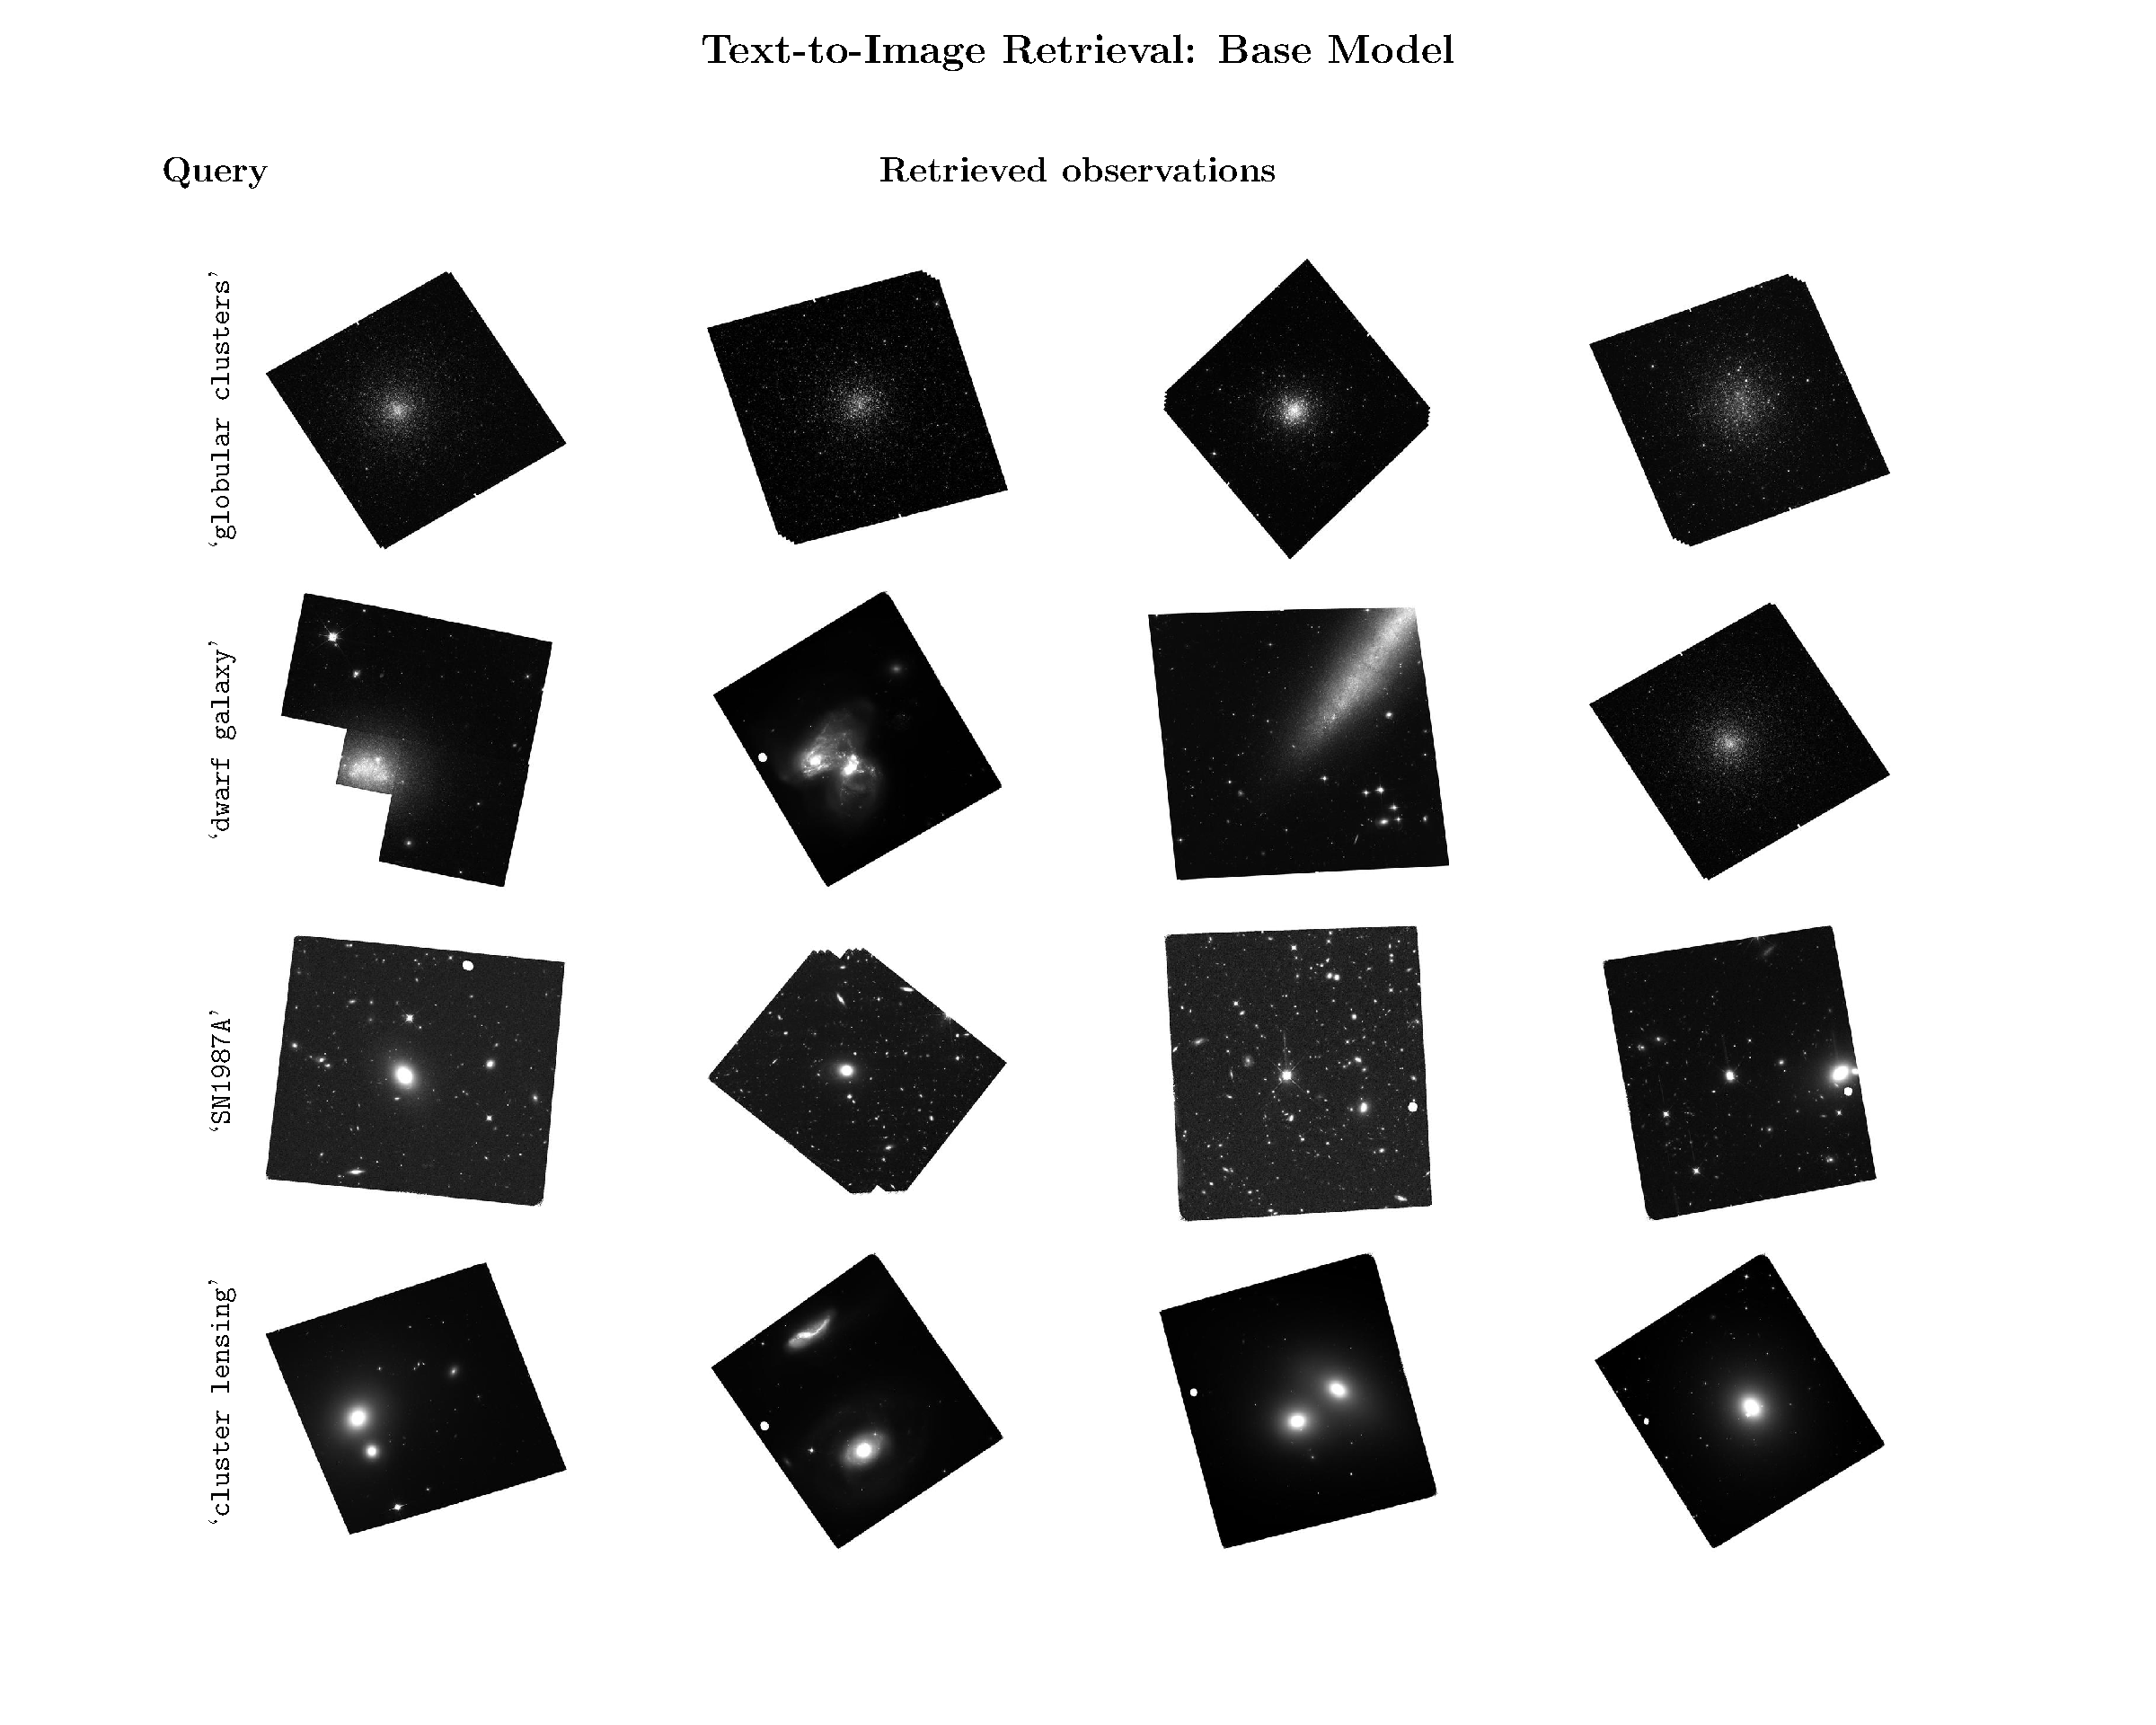
\includegraphics[width=0.95\textwidth]{plots/tti_base.pdf}
\caption{Retrieval accuracy}
\label{fig:tti}
\end{figure*}

\begin{figure*}[!h]
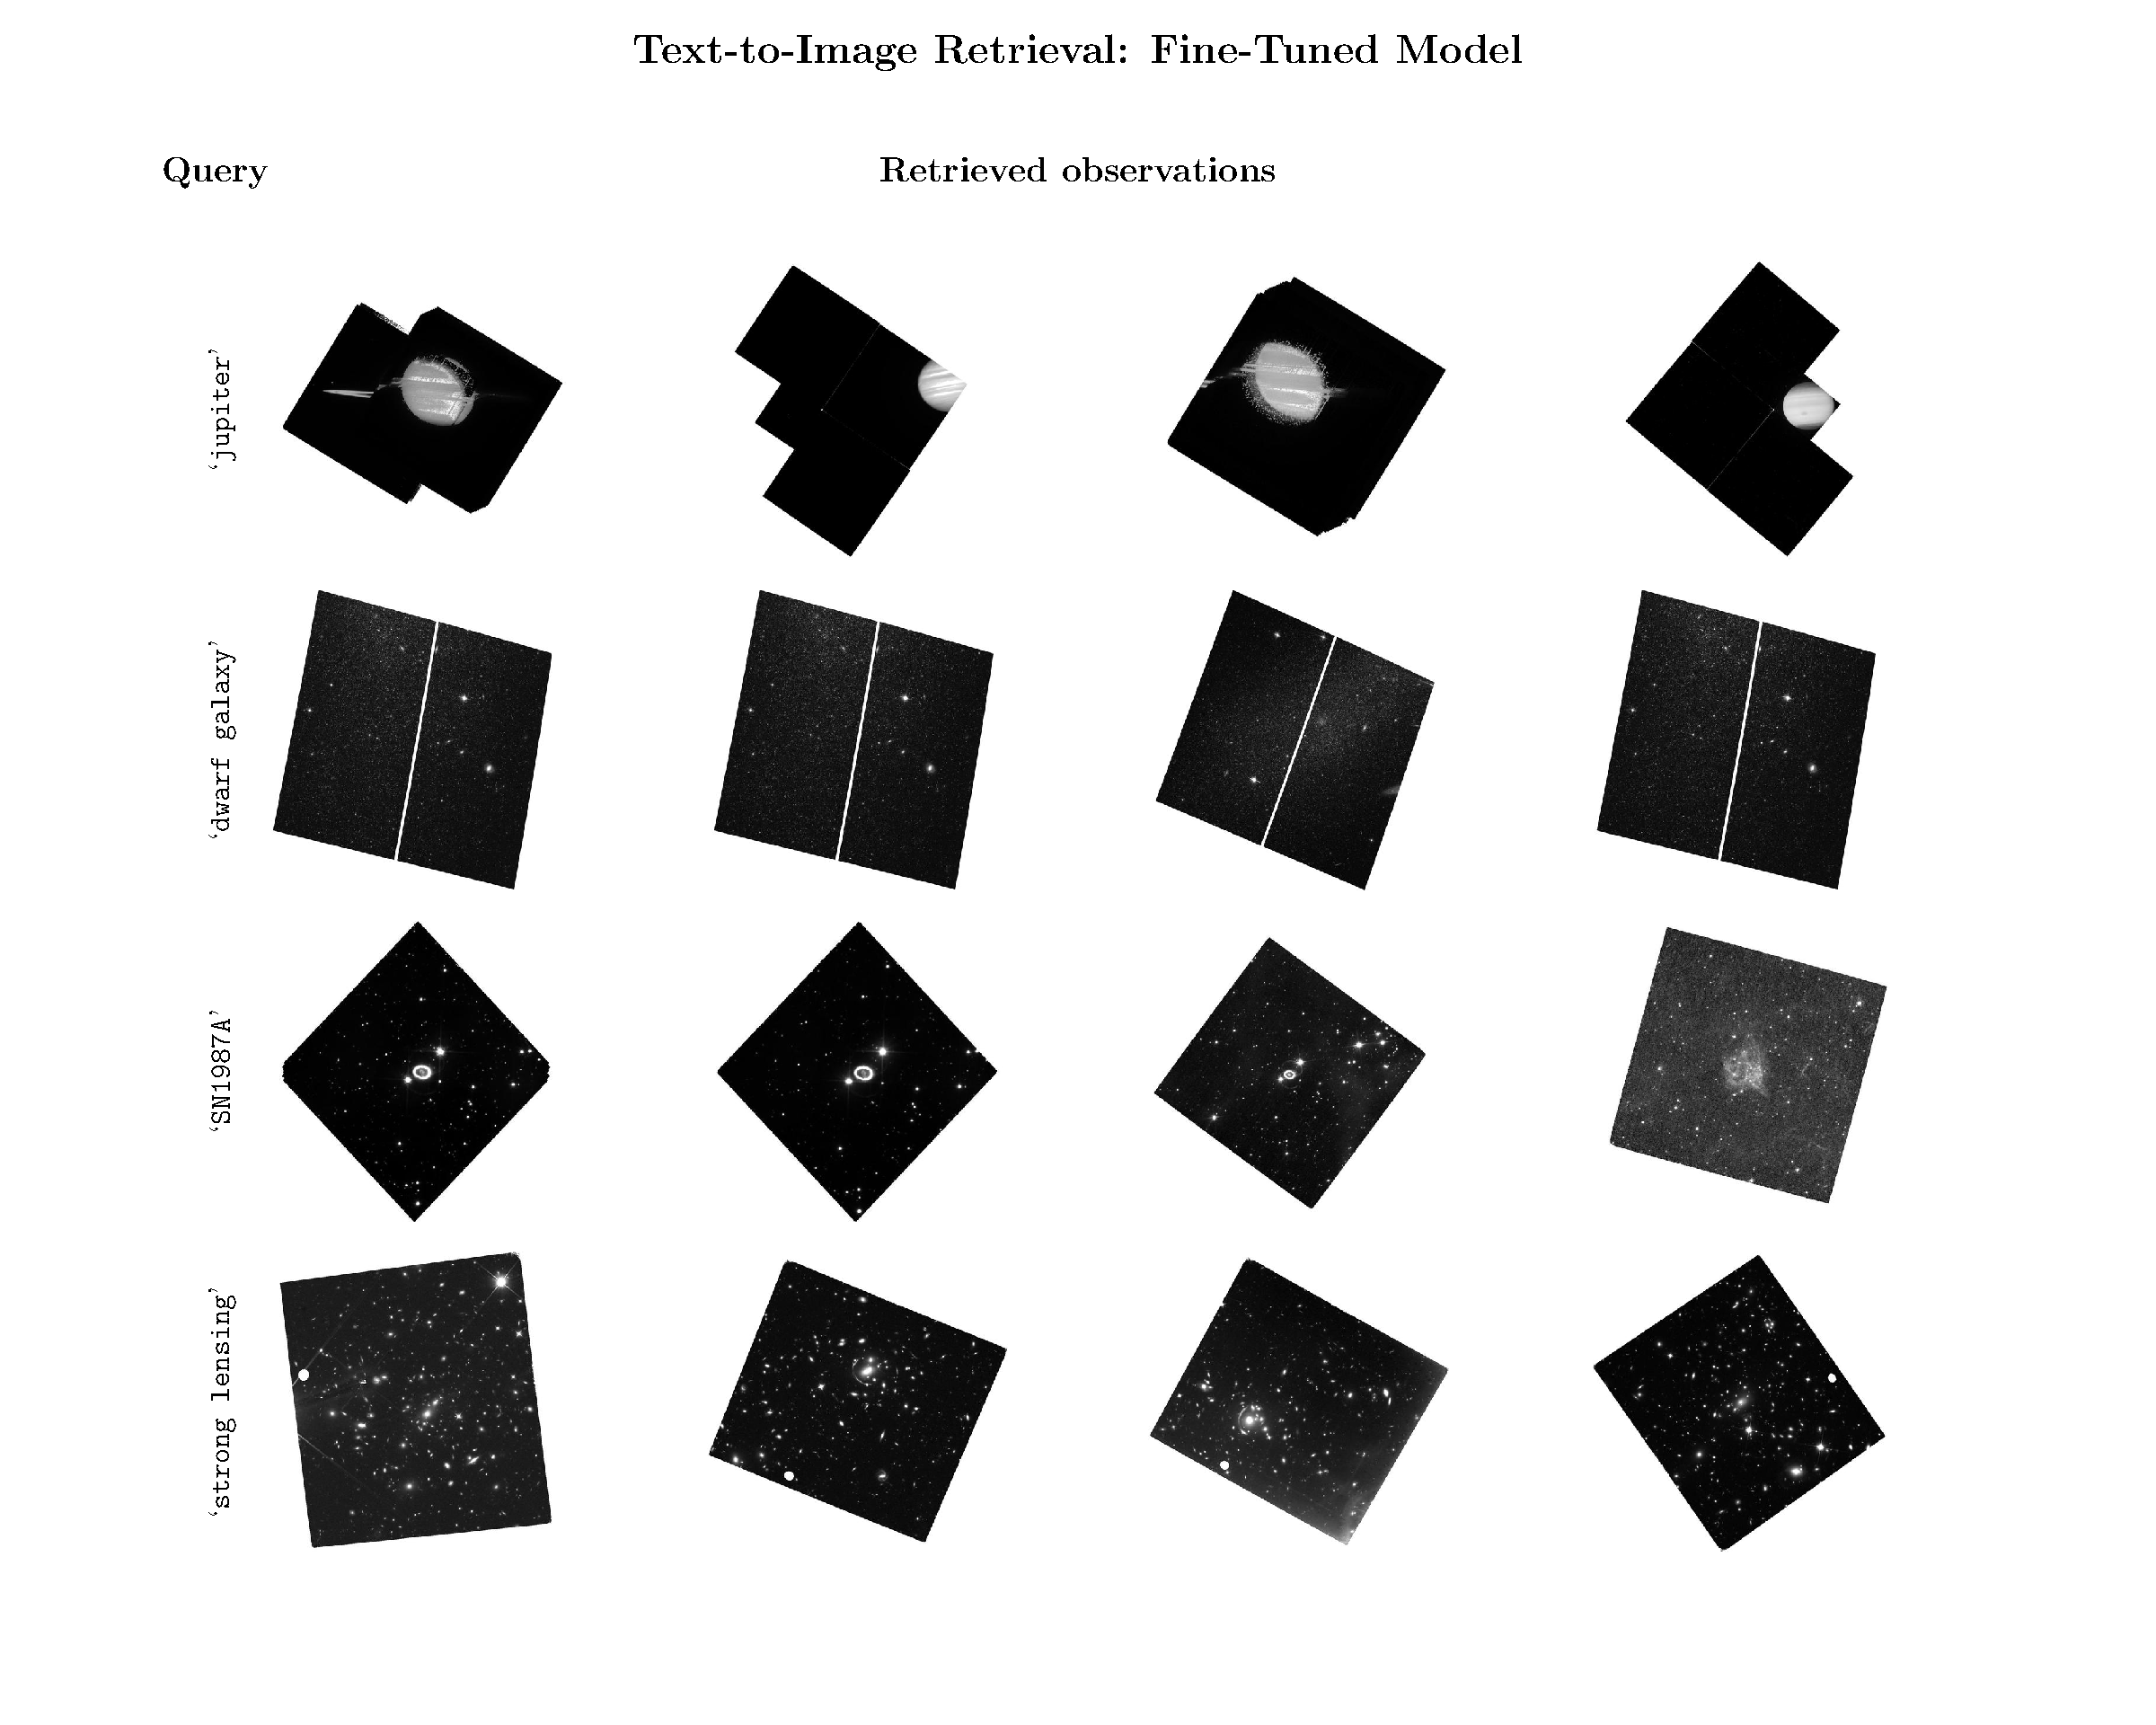
\includegraphics[width=0.95\textwidth]{plots/tti.pdf}
\caption{Retrieval accuracy}
\label{fig:tti_base}
\end{figure*}

% \subsubsection*{Broader Impact Statement}
% In this optional section, TMLR encourages authors to discuss possible repercussions of their work,
% notably any potential negative impact that a user of this research should be aware of. 
% Authors should consult the TMLR Ethics Guidelines available on the TMLR website
% for guidance on how to approach this subject.

% Should write BIS!

% \subsubsection*{Author Contributions}
% If you'd like to, you may include a section for author contributions as is done
% in many journals. This is optional and at the discretion of the authors. Only add
% this information once your submission is accepted and deanonymized. 

\subsubsection*{Code}

% Code repo and package cites.
% Dataset availability

\subsubsection*{Acknowledgments}
This work is supported by the National Science Foundation under Cooperative Agreement PHY-2019786 (The NSF AI Institute for Artificial Intelligence and Fundamental Interactions, \url{http://iaifi.org/}). This material is based upon work supported by the U.S. Department of Energy, Office of Science, Office of High Energy Physics of U.S. Department of Energy under grant Contract Number  DE-SC0012567. The computations in this paper were run on the FASRC Cannon cluster supported by the FAS Division of Science Research Computing Group at Harvard University.

This research is based on observations made with the NASA/ESA Hubble Space Telescope obtained from the Space Telescope Science Institute, which is operated by the Association of Universities for Research in Astronomy, Inc., under NASA contract NAS 5-26555.

Based on observations made with the NASA/ESA Hubble Space Telescope, and obtained from the Hubble Legacy Archive, which is a collaboration between the Space Telescope Science Institute (STScI/NASA), the Space Telescope European Coordinating Facility (ST-ECF/ESAC/ESA) and the Canadian Astronomy Data Centre (CADC/NRC/CSA).


\bibliography{main}
\bibliographystyle{tmlr}

\appendix
\section{Summarization via regex-guided generation}
\label{app:summarization}

The following prompt is used to summarize the abstracts.

\begin{lstlisting}[language=Python]
@outlines.prompt
def prompt_fn(abstract):
            
      """<s>[INST] You are an expert astrophysicist, with broad expertise across observational and theoretical astrophysics. You are able to extract core information from astrophysical texts.

Abstract: "{{abstract}}"

Based on the above observational proposal abstract, your task is to summarize the nature of the eventual observations. You will identify the astrophysical objects and phenomena, as well as the potential science use cases described in the abstract.

Follow these instructions exactly:
- Mention up to 5 items for both categories; do not mention more than 5 items in either category. 
- Choose the most relevant ones if there are more than 5 items in a category.
- Never mention the Hubble Space Telescope, HST, or the HST archive.
- Mention the class (e.g., barred spiral galaxy) and not just the specific instance (e.g., Andromeda).
- Name the objects in the science use cases, if appropriate.
- Write out full names of objects in addition to acronyms.
- Do not list irrelevant objects which do not describe the eventual observation, such as units or proposal Cycle numbers. List fewer but more relevant objects, if in doubt.
- Each science case listed must be self-contained but succinct.
- Only write in English.
- Do not list items that are too generic (e.g., galaxy, faint object, kinematics)
- The total length of text should not exceed 80 words.
- Present your lists in a comma-separated format; no dashed or numbered lists.

Example output: {'objects_and_phenomena':'spiral galaxies, galaxy clusters, supernova remnants', 'science_use_cases':'model galactic structure and evolution, characterize dark matter distribution in clusters, analyze expansion rates of supernova remnants'}

Answer in JSON format. The JSON should be a dictionary with keys "objects_and_phenomena" and "science_use_cases".

[/INST]
"""
\end{lstlisting}

\end{document}
